\documentclass[letterpaper,12pt]{article}
\usepackage[margin=14mm,top=18mm,bottom=17mm,headheight=14pt]{geometry}
\pdfmapfile{+cm.map}\pdfmapfile{+cmextra.map}
\usepackage{tikz,fancyhdr,amsmath,amssymb}
\usetikzlibrary{arrows.meta,patterns}
\pagestyle{fancy}\fancyhf{}\renewcommand{\headrulewidth}{0pt}
\fancyhead[L]{\small Week 51 / Honest measurement ranges / Grades 2--3}
\fancyfoot[L]{\small Bellingham Math Circle / Week 51 / F51-23-v2}
\fancyfoot[R]{\small\thepage}
\setlength{\parindent}{0pt}\setlength{\parskip}{0pt}
\begin{document}
\noindent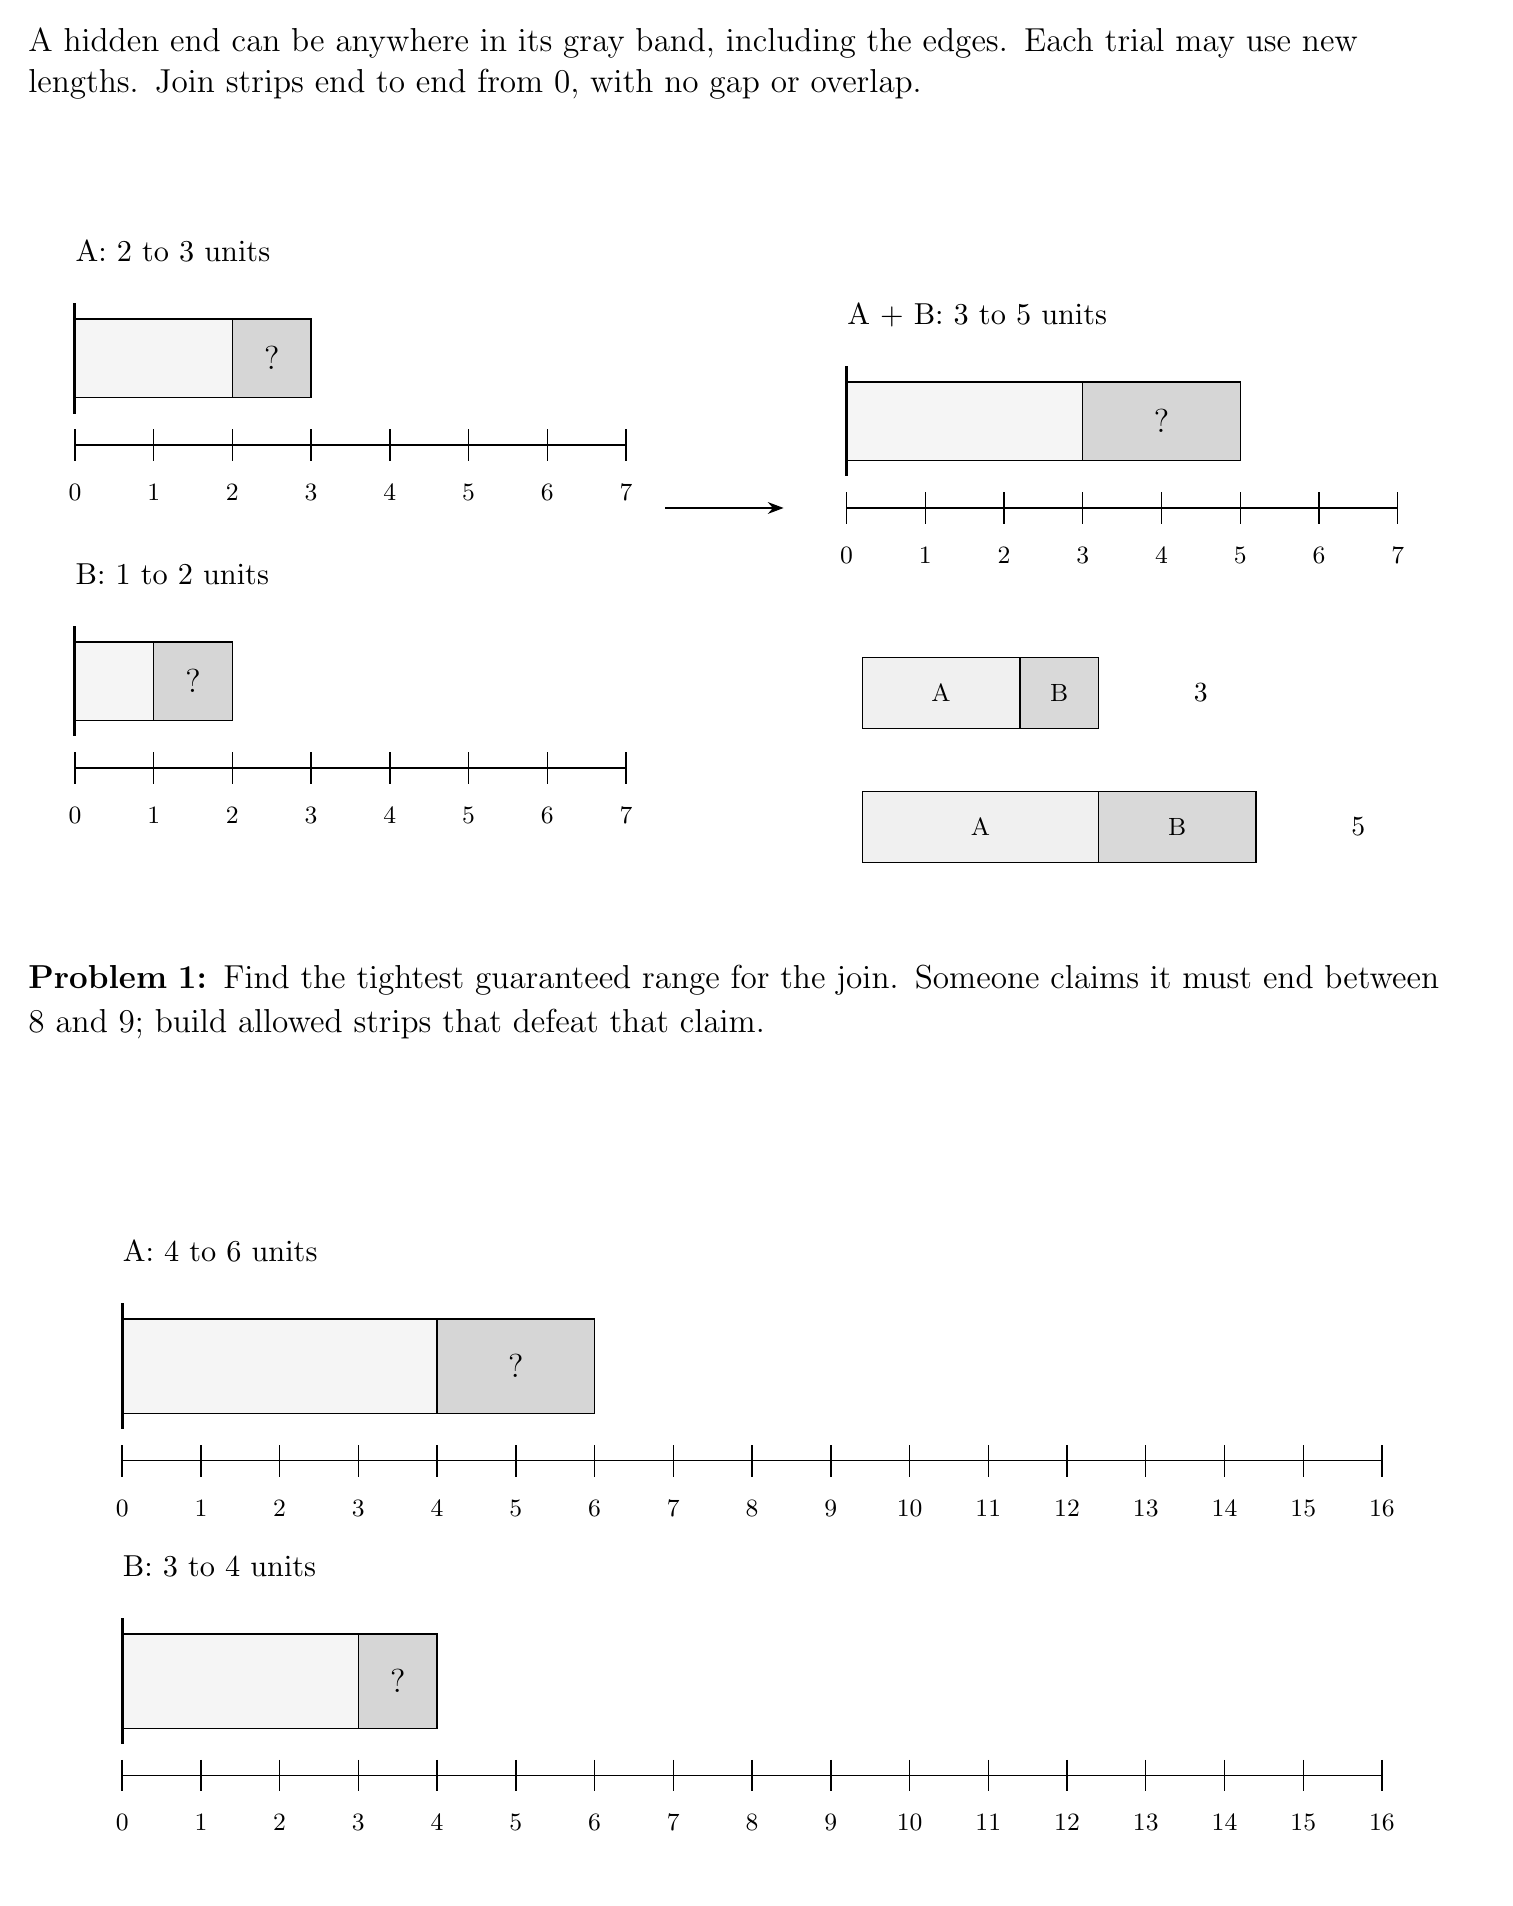
\begin{tikzpicture}[x=1mm,y=-1mm,line width=.5pt]
\path[use as bounding box] (0,0) rectangle (185,235);
\node[anchor=north west,inner sep=0pt,text width=180mm,font=\fontsize{12}{15}\selectfont] at (0,0) {A hidden end can be anywhere in its gray band, including the edges. Each trial may use new lengths. Join strips end to end from 0, with no gap or overlap.};
\draw[fill=gray!8] (6,37) rectangle ++(20,10);
\draw[fill=gray!32] (26,37) rectangle ++(10,10);
\draw[line width=1.1pt] (6,35) -- (6,49);
\node[anchor=center,inner sep=1pt,font=\fontsize{12}{14}\selectfont] at (31.0,42.0) {?};
\node[anchor=north west,inner sep=0pt,text width=80mm,font=\fontsize{11}{14}\selectfont] at (6,27) {A: 2 to 3 units};
\draw[] (6,53) -- (76,53);
\draw[] (6,51) -- (6,55);
\node[anchor=center,inner sep=1pt,font=\fontsize{9}{11}\selectfont] at (6,59) {0};
\draw[] (16,51) -- (16,55);
\node[anchor=center,inner sep=1pt,font=\fontsize{9}{11}\selectfont] at (16,59) {1};
\draw[] (26,51) -- (26,55);
\node[anchor=center,inner sep=1pt,font=\fontsize{9}{11}\selectfont] at (26,59) {2};
\draw[] (36,51) -- (36,55);
\node[anchor=center,inner sep=1pt,font=\fontsize{9}{11}\selectfont] at (36,59) {3};
\draw[] (46,51) -- (46,55);
\node[anchor=center,inner sep=1pt,font=\fontsize{9}{11}\selectfont] at (46,59) {4};
\draw[] (56,51) -- (56,55);
\node[anchor=center,inner sep=1pt,font=\fontsize{9}{11}\selectfont] at (56,59) {5};
\draw[] (66,51) -- (66,55);
\node[anchor=center,inner sep=1pt,font=\fontsize{9}{11}\selectfont] at (66,59) {6};
\draw[] (76,51) -- (76,55);
\node[anchor=center,inner sep=1pt,font=\fontsize{9}{11}\selectfont] at (76,59) {7};
\draw[fill=gray!8] (6,78) rectangle ++(10,10);
\draw[fill=gray!32] (16,78) rectangle ++(10,10);
\draw[line width=1.1pt] (6,76) -- (6,90);
\node[anchor=center,inner sep=1pt,font=\fontsize{12}{14}\selectfont] at (21.0,83.0) {?};
\node[anchor=north west,inner sep=0pt,text width=80mm,font=\fontsize{11}{14}\selectfont] at (6,68) {B: 1 to 2 units};
\draw[] (6,94) -- (76,94);
\draw[] (6,92) -- (6,96);
\node[anchor=center,inner sep=1pt,font=\fontsize{9}{11}\selectfont] at (6,100) {0};
\draw[] (16,92) -- (16,96);
\node[anchor=center,inner sep=1pt,font=\fontsize{9}{11}\selectfont] at (16,100) {1};
\draw[] (26,92) -- (26,96);
\node[anchor=center,inner sep=1pt,font=\fontsize{9}{11}\selectfont] at (26,100) {2};
\draw[] (36,92) -- (36,96);
\node[anchor=center,inner sep=1pt,font=\fontsize{9}{11}\selectfont] at (36,100) {3};
\draw[] (46,92) -- (46,96);
\node[anchor=center,inner sep=1pt,font=\fontsize{9}{11}\selectfont] at (46,100) {4};
\draw[] (56,92) -- (56,96);
\node[anchor=center,inner sep=1pt,font=\fontsize{9}{11}\selectfont] at (56,100) {5};
\draw[] (66,92) -- (66,96);
\node[anchor=center,inner sep=1pt,font=\fontsize{9}{11}\selectfont] at (66,100) {6};
\draw[] (76,92) -- (76,96);
\node[anchor=center,inner sep=1pt,font=\fontsize{9}{11}\selectfont] at (76,100) {7};
\draw[-{Stealth[length=2mm]}] (81,61) -- (96,61);
\draw[fill=gray!8] (104,45) rectangle ++(30,10);
\draw[fill=gray!32] (134,45) rectangle ++(20,10);
\draw[line width=1.1pt] (104,43) -- (104,57);
\node[anchor=center,inner sep=1pt,font=\fontsize{12}{14}\selectfont] at (144.0,50.0) {?};
\node[anchor=north west,inner sep=0pt,text width=76mm,font=\fontsize{11}{14}\selectfont] at (104,35) {A + B: 3 to 5 units};
\draw[] (104,61) -- (174,61);
\draw[] (104,59) -- (104,63);
\node[anchor=center,inner sep=1pt,font=\fontsize{9}{11}\selectfont] at (104,67) {0};
\draw[] (114,59) -- (114,63);
\node[anchor=center,inner sep=1pt,font=\fontsize{9}{11}\selectfont] at (114,67) {1};
\draw[] (124,59) -- (124,63);
\node[anchor=center,inner sep=1pt,font=\fontsize{9}{11}\selectfont] at (124,67) {2};
\draw[] (134,59) -- (134,63);
\node[anchor=center,inner sep=1pt,font=\fontsize{9}{11}\selectfont] at (134,67) {3};
\draw[] (144,59) -- (144,63);
\node[anchor=center,inner sep=1pt,font=\fontsize{9}{11}\selectfont] at (144,67) {4};
\draw[] (154,59) -- (154,63);
\node[anchor=center,inner sep=1pt,font=\fontsize{9}{11}\selectfont] at (154,67) {5};
\draw[] (164,59) -- (164,63);
\node[anchor=center,inner sep=1pt,font=\fontsize{9}{11}\selectfont] at (164,67) {6};
\draw[] (174,59) -- (174,63);
\node[anchor=center,inner sep=1pt,font=\fontsize{9}{11}\selectfont] at (174,67) {7};
\draw[fill=gray!12] (106,80) rectangle ++(20,9);
\node[anchor=center,inner sep=1pt,font=\fontsize{9}{11}\selectfont] at (116.0,84.5) {A};
\draw[fill=gray!30] (126,80) rectangle ++(10,9);
\node[anchor=center,inner sep=1pt,font=\fontsize{9}{11}\selectfont] at (131.0,84.5) {B};
\node[anchor=center,inner sep=1pt,font=\fontsize{10}{12}\selectfont] at (149,84.5) {3};
\draw[fill=gray!12] (106,97) rectangle ++(30,9);
\node[anchor=center,inner sep=1pt,font=\fontsize{9}{11}\selectfont] at (121.0,101.5) {A};
\draw[fill=gray!30] (136,97) rectangle ++(20,9);
\node[anchor=center,inner sep=1pt,font=\fontsize{9}{11}\selectfont] at (146.0,101.5) {B};
\node[anchor=center,inner sep=1pt,font=\fontsize{10}{12}\selectfont] at (169,101.5) {5};
\node[anchor=north west,inner sep=0pt,text width=180mm,font=\fontsize{13}{16}\selectfont] at (0,119) {\textbf{Problem 1:} Find the tightest guaranteed range for the join. Someone claims it must end between 8 and 9; build allowed strips that defeat that claim.};
\draw[fill=gray!8] (12,164) rectangle ++(40,12);
\draw[fill=gray!32] (52,164) rectangle ++(20,12);
\draw[line width=1.1pt] (12,162) -- (12,178);
\node[anchor=center,inner sep=1pt,font=\fontsize{12}{14}\selectfont] at (62.0,170.0) {?};
\node[anchor=north west,inner sep=0pt,text width=168mm,font=\fontsize{11}{14}\selectfont] at (12,154) {A: 4 to 6 units};
\draw[] (12,182) -- (172,182);
\draw[] (12,180) -- (12,184);
\node[anchor=center,inner sep=1pt,font=\fontsize{9}{11}\selectfont] at (12,188) {0};
\draw[] (22,180) -- (22,184);
\node[anchor=center,inner sep=1pt,font=\fontsize{9}{11}\selectfont] at (22,188) {1};
\draw[] (32,180) -- (32,184);
\node[anchor=center,inner sep=1pt,font=\fontsize{9}{11}\selectfont] at (32,188) {2};
\draw[] (42,180) -- (42,184);
\node[anchor=center,inner sep=1pt,font=\fontsize{9}{11}\selectfont] at (42,188) {3};
\draw[] (52,180) -- (52,184);
\node[anchor=center,inner sep=1pt,font=\fontsize{9}{11}\selectfont] at (52,188) {4};
\draw[] (62,180) -- (62,184);
\node[anchor=center,inner sep=1pt,font=\fontsize{9}{11}\selectfont] at (62,188) {5};
\draw[] (72,180) -- (72,184);
\node[anchor=center,inner sep=1pt,font=\fontsize{9}{11}\selectfont] at (72,188) {6};
\draw[] (82,180) -- (82,184);
\node[anchor=center,inner sep=1pt,font=\fontsize{9}{11}\selectfont] at (82,188) {7};
\draw[] (92,180) -- (92,184);
\node[anchor=center,inner sep=1pt,font=\fontsize{9}{11}\selectfont] at (92,188) {8};
\draw[] (102,180) -- (102,184);
\node[anchor=center,inner sep=1pt,font=\fontsize{9}{11}\selectfont] at (102,188) {9};
\draw[] (112,180) -- (112,184);
\node[anchor=center,inner sep=1pt,font=\fontsize{9}{11}\selectfont] at (112,188) {10};
\draw[] (122,180) -- (122,184);
\node[anchor=center,inner sep=1pt,font=\fontsize{9}{11}\selectfont] at (122,188) {11};
\draw[] (132,180) -- (132,184);
\node[anchor=center,inner sep=1pt,font=\fontsize{9}{11}\selectfont] at (132,188) {12};
\draw[] (142,180) -- (142,184);
\node[anchor=center,inner sep=1pt,font=\fontsize{9}{11}\selectfont] at (142,188) {13};
\draw[] (152,180) -- (152,184);
\node[anchor=center,inner sep=1pt,font=\fontsize{9}{11}\selectfont] at (152,188) {14};
\draw[] (162,180) -- (162,184);
\node[anchor=center,inner sep=1pt,font=\fontsize{9}{11}\selectfont] at (162,188) {15};
\draw[] (172,180) -- (172,184);
\node[anchor=center,inner sep=1pt,font=\fontsize{9}{11}\selectfont] at (172,188) {16};
\draw[fill=gray!8] (12,204) rectangle ++(30,12);
\draw[fill=gray!32] (42,204) rectangle ++(10,12);
\draw[line width=1.1pt] (12,202) -- (12,218);
\node[anchor=center,inner sep=1pt,font=\fontsize{12}{14}\selectfont] at (47.0,210.0) {?};
\node[anchor=north west,inner sep=0pt,text width=168mm,font=\fontsize{11}{14}\selectfont] at (12,194) {B: 3 to 4 units};
\draw[] (12,222) -- (172,222);
\draw[] (12,220) -- (12,224);
\node[anchor=center,inner sep=1pt,font=\fontsize{9}{11}\selectfont] at (12,228) {0};
\draw[] (22,220) -- (22,224);
\node[anchor=center,inner sep=1pt,font=\fontsize{9}{11}\selectfont] at (22,228) {1};
\draw[] (32,220) -- (32,224);
\node[anchor=center,inner sep=1pt,font=\fontsize{9}{11}\selectfont] at (32,228) {2};
\draw[] (42,220) -- (42,224);
\node[anchor=center,inner sep=1pt,font=\fontsize{9}{11}\selectfont] at (42,228) {3};
\draw[] (52,220) -- (52,224);
\node[anchor=center,inner sep=1pt,font=\fontsize{9}{11}\selectfont] at (52,228) {4};
\draw[] (62,220) -- (62,224);
\node[anchor=center,inner sep=1pt,font=\fontsize{9}{11}\selectfont] at (62,228) {5};
\draw[] (72,220) -- (72,224);
\node[anchor=center,inner sep=1pt,font=\fontsize{9}{11}\selectfont] at (72,228) {6};
\draw[] (82,220) -- (82,224);
\node[anchor=center,inner sep=1pt,font=\fontsize{9}{11}\selectfont] at (82,228) {7};
\draw[] (92,220) -- (92,224);
\node[anchor=center,inner sep=1pt,font=\fontsize{9}{11}\selectfont] at (92,228) {8};
\draw[] (102,220) -- (102,224);
\node[anchor=center,inner sep=1pt,font=\fontsize{9}{11}\selectfont] at (102,228) {9};
\draw[] (112,220) -- (112,224);
\node[anchor=center,inner sep=1pt,font=\fontsize{9}{11}\selectfont] at (112,228) {10};
\draw[] (122,220) -- (122,224);
\node[anchor=center,inner sep=1pt,font=\fontsize{9}{11}\selectfont] at (122,228) {11};
\draw[] (132,220) -- (132,224);
\node[anchor=center,inner sep=1pt,font=\fontsize{9}{11}\selectfont] at (132,228) {12};
\draw[] (142,220) -- (142,224);
\node[anchor=center,inner sep=1pt,font=\fontsize{9}{11}\selectfont] at (142,228) {13};
\draw[] (152,220) -- (152,224);
\node[anchor=center,inner sep=1pt,font=\fontsize{9}{11}\selectfont] at (152,228) {14};
\draw[] (162,220) -- (162,224);
\node[anchor=center,inner sep=1pt,font=\fontsize{9}{11}\selectfont] at (162,228) {15};
\draw[] (172,220) -- (172,224);
\node[anchor=center,inner sep=1pt,font=\fontsize{9}{11}\selectfont] at (172,228) {16};
\end{tikzpicture}
\newpage
\noindent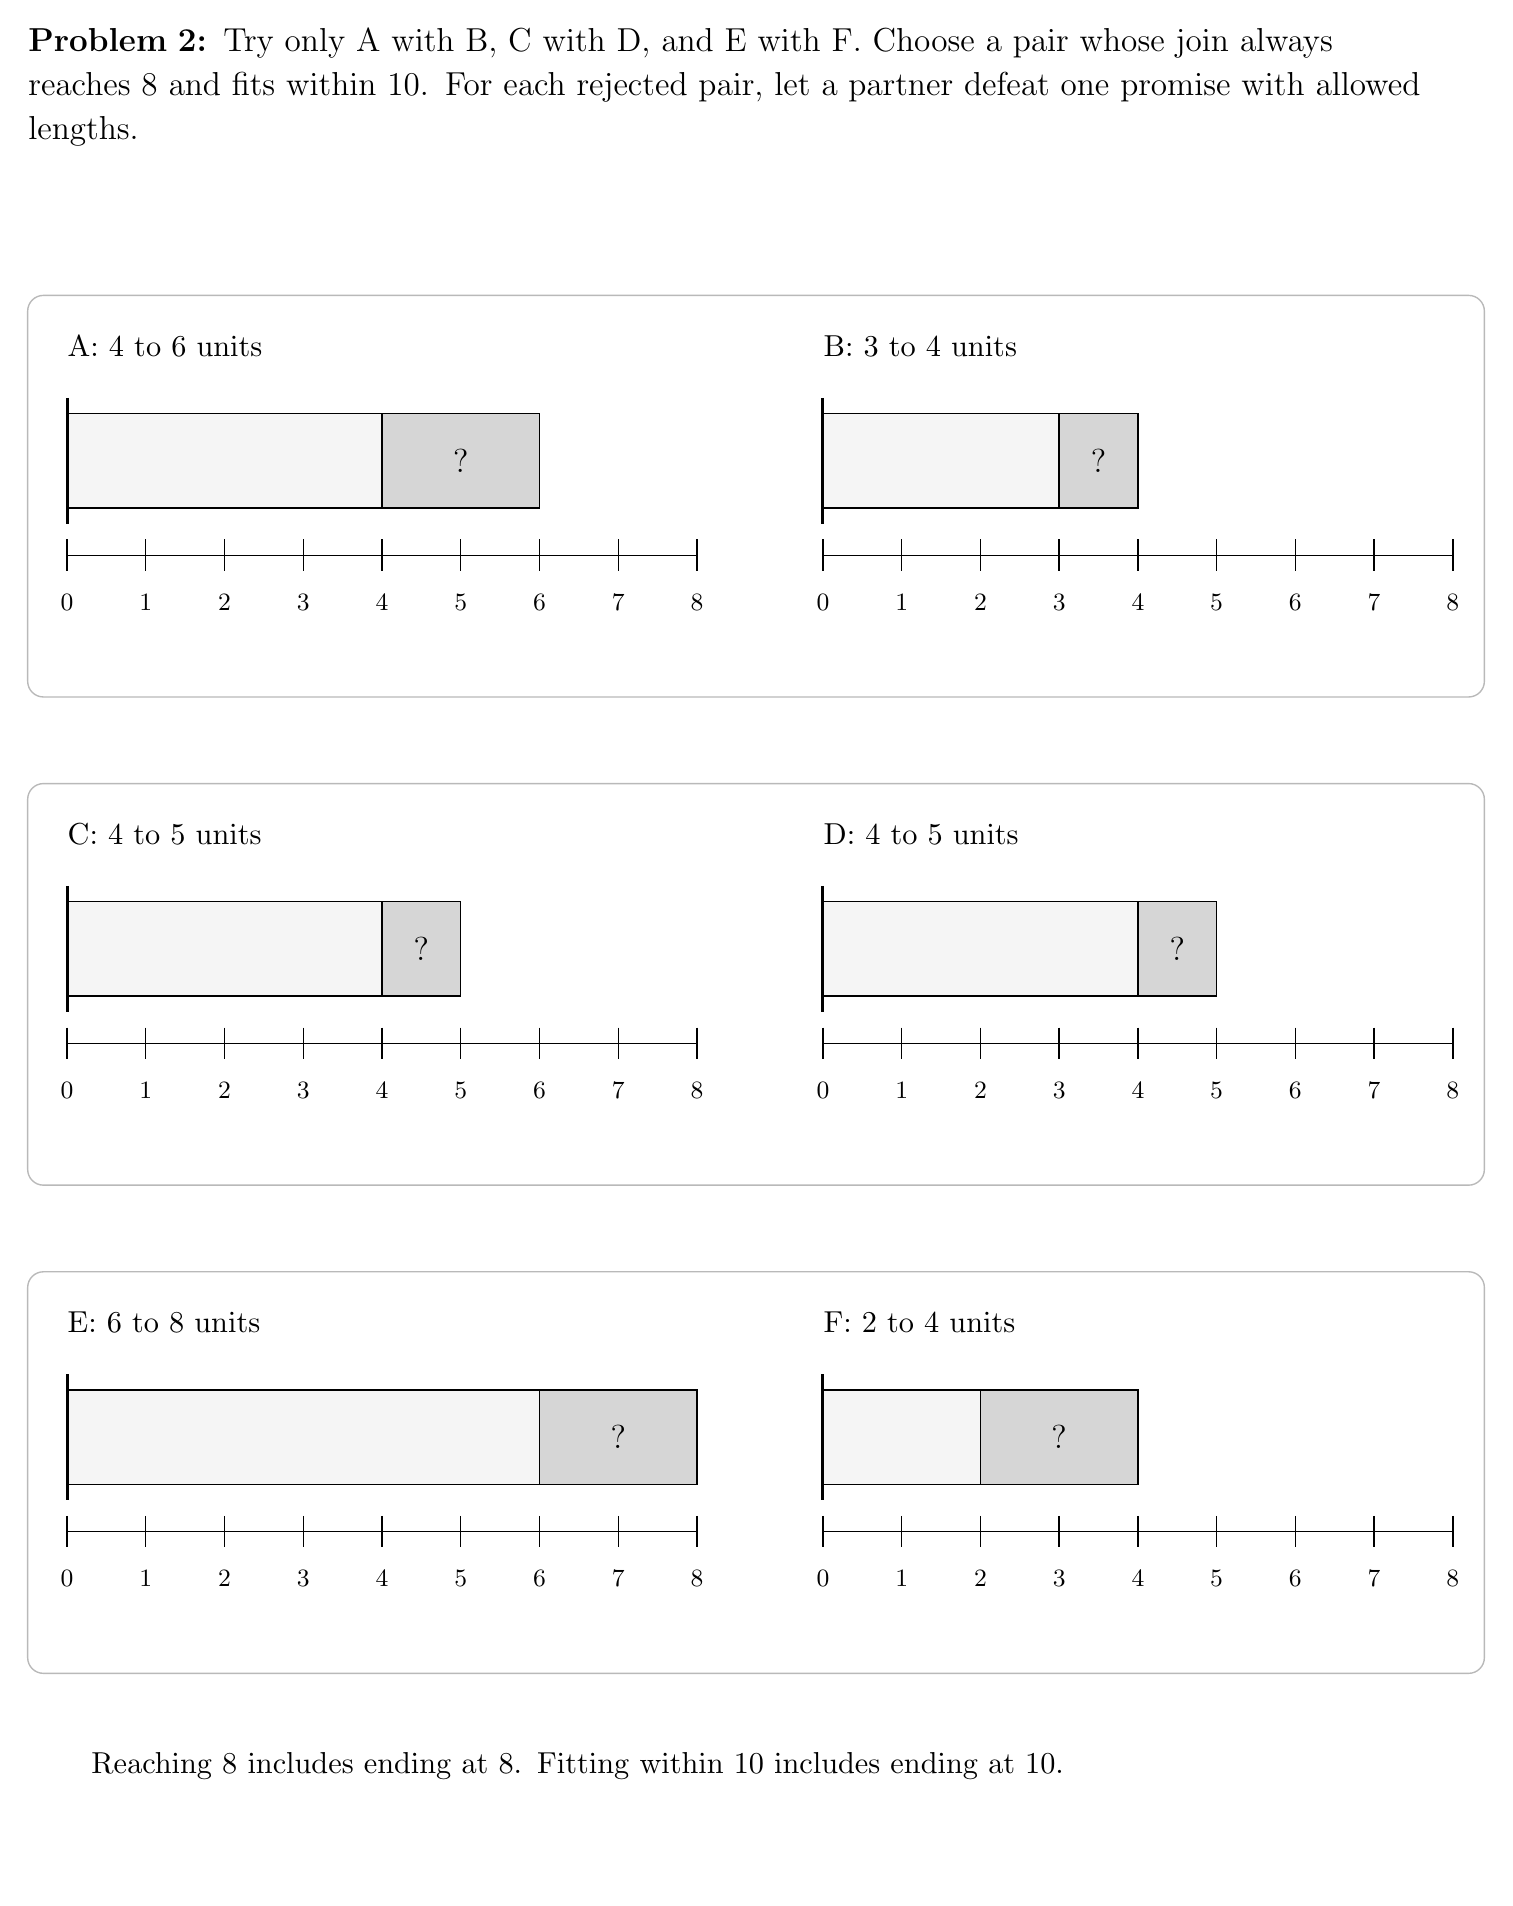
\begin{tikzpicture}[x=1mm,y=-1mm,line width=.5pt]
\path[use as bounding box] (0,0) rectangle (185,235);
\node[anchor=north west,inner sep=0pt,text width=180mm,font=\fontsize{13}{16}\selectfont] at (0,0) {\textbf{Problem 2:} Try only A with B, C with D, and E with F. Choose a pair whose join always reaches 8 and fits within 10. For each rejected pair, let a partner defeat one promise with allowed lengths.};
\draw[rounded corners=2mm,gray!55] (0,34) rectangle ++(185,51);
\draw[fill=gray!8] (5,49) rectangle ++(40,12);
\draw[fill=gray!32] (45,49) rectangle ++(20,12);
\draw[line width=1.1pt] (5,47) -- (5,63);
\node[anchor=center,inner sep=1pt,font=\fontsize{12}{14}\selectfont] at (55.0,55.0) {?};
\node[anchor=north west,inner sep=0pt,text width=90mm,font=\fontsize{11}{14}\selectfont] at (5,39) {A: 4 to 6 units};
\draw[] (5,67) -- (85,67);
\draw[] (5,65) -- (5,69);
\node[anchor=center,inner sep=1pt,font=\fontsize{9}{11}\selectfont] at (5,73) {0};
\draw[] (15,65) -- (15,69);
\node[anchor=center,inner sep=1pt,font=\fontsize{9}{11}\selectfont] at (15,73) {1};
\draw[] (25,65) -- (25,69);
\node[anchor=center,inner sep=1pt,font=\fontsize{9}{11}\selectfont] at (25,73) {2};
\draw[] (35,65) -- (35,69);
\node[anchor=center,inner sep=1pt,font=\fontsize{9}{11}\selectfont] at (35,73) {3};
\draw[] (45,65) -- (45,69);
\node[anchor=center,inner sep=1pt,font=\fontsize{9}{11}\selectfont] at (45,73) {4};
\draw[] (55,65) -- (55,69);
\node[anchor=center,inner sep=1pt,font=\fontsize{9}{11}\selectfont] at (55,73) {5};
\draw[] (65,65) -- (65,69);
\node[anchor=center,inner sep=1pt,font=\fontsize{9}{11}\selectfont] at (65,73) {6};
\draw[] (75,65) -- (75,69);
\node[anchor=center,inner sep=1pt,font=\fontsize{9}{11}\selectfont] at (75,73) {7};
\draw[] (85,65) -- (85,69);
\node[anchor=center,inner sep=1pt,font=\fontsize{9}{11}\selectfont] at (85,73) {8};
\draw[fill=gray!8] (101,49) rectangle ++(30,12);
\draw[fill=gray!32] (131,49) rectangle ++(10,12);
\draw[line width=1.1pt] (101,47) -- (101,63);
\node[anchor=center,inner sep=1pt,font=\fontsize{12}{14}\selectfont] at (136.0,55.0) {?};
\node[anchor=north west,inner sep=0pt,text width=79mm,font=\fontsize{11}{14}\selectfont] at (101,39) {B: 3 to 4 units};
\draw[] (101,67) -- (181,67);
\draw[] (101,65) -- (101,69);
\node[anchor=center,inner sep=1pt,font=\fontsize{9}{11}\selectfont] at (101,73) {0};
\draw[] (111,65) -- (111,69);
\node[anchor=center,inner sep=1pt,font=\fontsize{9}{11}\selectfont] at (111,73) {1};
\draw[] (121,65) -- (121,69);
\node[anchor=center,inner sep=1pt,font=\fontsize{9}{11}\selectfont] at (121,73) {2};
\draw[] (131,65) -- (131,69);
\node[anchor=center,inner sep=1pt,font=\fontsize{9}{11}\selectfont] at (131,73) {3};
\draw[] (141,65) -- (141,69);
\node[anchor=center,inner sep=1pt,font=\fontsize{9}{11}\selectfont] at (141,73) {4};
\draw[] (151,65) -- (151,69);
\node[anchor=center,inner sep=1pt,font=\fontsize{9}{11}\selectfont] at (151,73) {5};
\draw[] (161,65) -- (161,69);
\node[anchor=center,inner sep=1pt,font=\fontsize{9}{11}\selectfont] at (161,73) {6};
\draw[] (171,65) -- (171,69);
\node[anchor=center,inner sep=1pt,font=\fontsize{9}{11}\selectfont] at (171,73) {7};
\draw[] (181,65) -- (181,69);
\node[anchor=center,inner sep=1pt,font=\fontsize{9}{11}\selectfont] at (181,73) {8};
\draw[rounded corners=2mm,gray!55] (0,96) rectangle ++(185,51);
\draw[fill=gray!8] (5,111) rectangle ++(40,12);
\draw[fill=gray!32] (45,111) rectangle ++(10,12);
\draw[line width=1.1pt] (5,109) -- (5,125);
\node[anchor=center,inner sep=1pt,font=\fontsize{12}{14}\selectfont] at (50.0,117.0) {?};
\node[anchor=north west,inner sep=0pt,text width=90mm,font=\fontsize{11}{14}\selectfont] at (5,101) {C: 4 to 5 units};
\draw[] (5,129) -- (85,129);
\draw[] (5,127) -- (5,131);
\node[anchor=center,inner sep=1pt,font=\fontsize{9}{11}\selectfont] at (5,135) {0};
\draw[] (15,127) -- (15,131);
\node[anchor=center,inner sep=1pt,font=\fontsize{9}{11}\selectfont] at (15,135) {1};
\draw[] (25,127) -- (25,131);
\node[anchor=center,inner sep=1pt,font=\fontsize{9}{11}\selectfont] at (25,135) {2};
\draw[] (35,127) -- (35,131);
\node[anchor=center,inner sep=1pt,font=\fontsize{9}{11}\selectfont] at (35,135) {3};
\draw[] (45,127) -- (45,131);
\node[anchor=center,inner sep=1pt,font=\fontsize{9}{11}\selectfont] at (45,135) {4};
\draw[] (55,127) -- (55,131);
\node[anchor=center,inner sep=1pt,font=\fontsize{9}{11}\selectfont] at (55,135) {5};
\draw[] (65,127) -- (65,131);
\node[anchor=center,inner sep=1pt,font=\fontsize{9}{11}\selectfont] at (65,135) {6};
\draw[] (75,127) -- (75,131);
\node[anchor=center,inner sep=1pt,font=\fontsize{9}{11}\selectfont] at (75,135) {7};
\draw[] (85,127) -- (85,131);
\node[anchor=center,inner sep=1pt,font=\fontsize{9}{11}\selectfont] at (85,135) {8};
\draw[fill=gray!8] (101,111) rectangle ++(40,12);
\draw[fill=gray!32] (141,111) rectangle ++(10,12);
\draw[line width=1.1pt] (101,109) -- (101,125);
\node[anchor=center,inner sep=1pt,font=\fontsize{12}{14}\selectfont] at (146.0,117.0) {?};
\node[anchor=north west,inner sep=0pt,text width=79mm,font=\fontsize{11}{14}\selectfont] at (101,101) {D: 4 to 5 units};
\draw[] (101,129) -- (181,129);
\draw[] (101,127) -- (101,131);
\node[anchor=center,inner sep=1pt,font=\fontsize{9}{11}\selectfont] at (101,135) {0};
\draw[] (111,127) -- (111,131);
\node[anchor=center,inner sep=1pt,font=\fontsize{9}{11}\selectfont] at (111,135) {1};
\draw[] (121,127) -- (121,131);
\node[anchor=center,inner sep=1pt,font=\fontsize{9}{11}\selectfont] at (121,135) {2};
\draw[] (131,127) -- (131,131);
\node[anchor=center,inner sep=1pt,font=\fontsize{9}{11}\selectfont] at (131,135) {3};
\draw[] (141,127) -- (141,131);
\node[anchor=center,inner sep=1pt,font=\fontsize{9}{11}\selectfont] at (141,135) {4};
\draw[] (151,127) -- (151,131);
\node[anchor=center,inner sep=1pt,font=\fontsize{9}{11}\selectfont] at (151,135) {5};
\draw[] (161,127) -- (161,131);
\node[anchor=center,inner sep=1pt,font=\fontsize{9}{11}\selectfont] at (161,135) {6};
\draw[] (171,127) -- (171,131);
\node[anchor=center,inner sep=1pt,font=\fontsize{9}{11}\selectfont] at (171,135) {7};
\draw[] (181,127) -- (181,131);
\node[anchor=center,inner sep=1pt,font=\fontsize{9}{11}\selectfont] at (181,135) {8};
\draw[rounded corners=2mm,gray!55] (0,158) rectangle ++(185,51);
\draw[fill=gray!8] (5,173) rectangle ++(60,12);
\draw[fill=gray!32] (65,173) rectangle ++(20,12);
\draw[line width=1.1pt] (5,171) -- (5,187);
\node[anchor=center,inner sep=1pt,font=\fontsize{12}{14}\selectfont] at (75.0,179.0) {?};
\node[anchor=north west,inner sep=0pt,text width=90mm,font=\fontsize{11}{14}\selectfont] at (5,163) {E: 6 to 8 units};
\draw[] (5,191) -- (85,191);
\draw[] (5,189) -- (5,193);
\node[anchor=center,inner sep=1pt,font=\fontsize{9}{11}\selectfont] at (5,197) {0};
\draw[] (15,189) -- (15,193);
\node[anchor=center,inner sep=1pt,font=\fontsize{9}{11}\selectfont] at (15,197) {1};
\draw[] (25,189) -- (25,193);
\node[anchor=center,inner sep=1pt,font=\fontsize{9}{11}\selectfont] at (25,197) {2};
\draw[] (35,189) -- (35,193);
\node[anchor=center,inner sep=1pt,font=\fontsize{9}{11}\selectfont] at (35,197) {3};
\draw[] (45,189) -- (45,193);
\node[anchor=center,inner sep=1pt,font=\fontsize{9}{11}\selectfont] at (45,197) {4};
\draw[] (55,189) -- (55,193);
\node[anchor=center,inner sep=1pt,font=\fontsize{9}{11}\selectfont] at (55,197) {5};
\draw[] (65,189) -- (65,193);
\node[anchor=center,inner sep=1pt,font=\fontsize{9}{11}\selectfont] at (65,197) {6};
\draw[] (75,189) -- (75,193);
\node[anchor=center,inner sep=1pt,font=\fontsize{9}{11}\selectfont] at (75,197) {7};
\draw[] (85,189) -- (85,193);
\node[anchor=center,inner sep=1pt,font=\fontsize{9}{11}\selectfont] at (85,197) {8};
\draw[fill=gray!8] (101,173) rectangle ++(20,12);
\draw[fill=gray!32] (121,173) rectangle ++(20,12);
\draw[line width=1.1pt] (101,171) -- (101,187);
\node[anchor=center,inner sep=1pt,font=\fontsize{12}{14}\selectfont] at (131.0,179.0) {?};
\node[anchor=north west,inner sep=0pt,text width=79mm,font=\fontsize{11}{14}\selectfont] at (101,163) {F: 2 to 4 units};
\draw[] (101,191) -- (181,191);
\draw[] (101,189) -- (101,193);
\node[anchor=center,inner sep=1pt,font=\fontsize{9}{11}\selectfont] at (101,197) {0};
\draw[] (111,189) -- (111,193);
\node[anchor=center,inner sep=1pt,font=\fontsize{9}{11}\selectfont] at (111,197) {1};
\draw[] (121,189) -- (121,193);
\node[anchor=center,inner sep=1pt,font=\fontsize{9}{11}\selectfont] at (121,197) {2};
\draw[] (131,189) -- (131,193);
\node[anchor=center,inner sep=1pt,font=\fontsize{9}{11}\selectfont] at (131,197) {3};
\draw[] (141,189) -- (141,193);
\node[anchor=center,inner sep=1pt,font=\fontsize{9}{11}\selectfont] at (141,197) {4};
\draw[] (151,189) -- (151,193);
\node[anchor=center,inner sep=1pt,font=\fontsize{9}{11}\selectfont] at (151,197) {5};
\draw[] (161,189) -- (161,193);
\node[anchor=center,inner sep=1pt,font=\fontsize{9}{11}\selectfont] at (161,197) {6};
\draw[] (171,189) -- (171,193);
\node[anchor=center,inner sep=1pt,font=\fontsize{9}{11}\selectfont] at (171,197) {7};
\draw[] (181,189) -- (181,193);
\node[anchor=center,inner sep=1pt,font=\fontsize{9}{11}\selectfont] at (181,197) {8};
\node[anchor=north west,inner sep=0pt,text width=178mm,font=\fontsize{11}{14}\selectfont] at (8,219) {Reaching 8 includes ending at 8. Fitting within 10 includes ending at 10.};
\end{tikzpicture}
\newpage
\noindent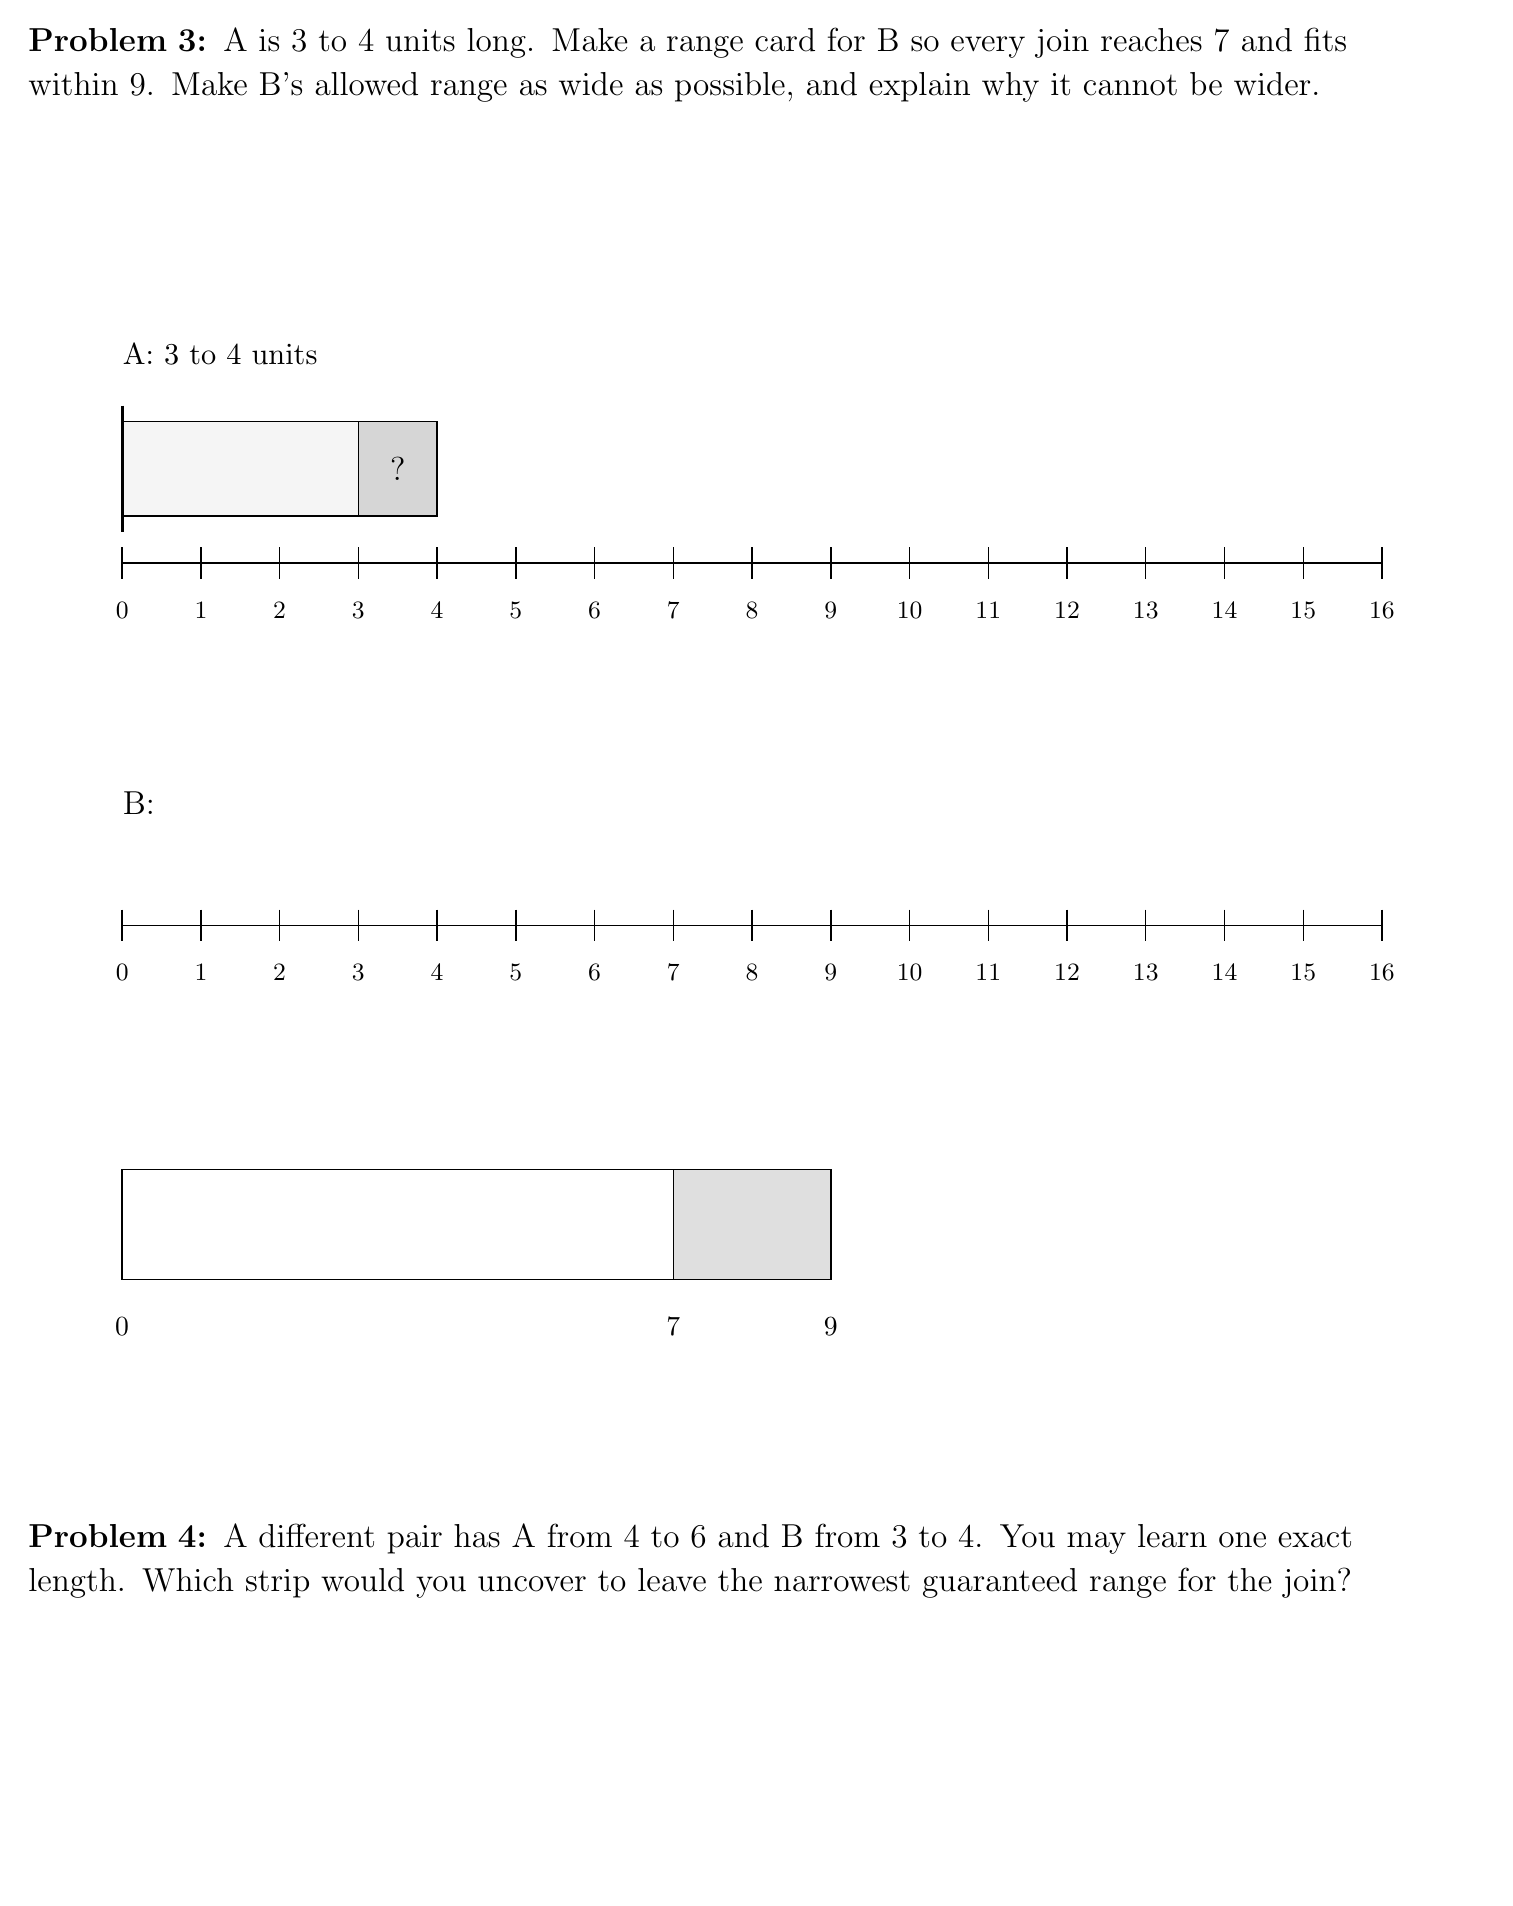
\begin{tikzpicture}[x=1mm,y=-1mm,line width=.5pt]
\path[use as bounding box] (0,0) rectangle (185,235);
\node[anchor=north west,inner sep=0pt,text width=180mm,font=\fontsize{13}{16}\selectfont] at (0,0) {\textbf{Problem 3:} A is 3 to 4 units long. Make a range card for B so every join reaches 7 and fits within 9. Make B's allowed range as wide as possible, and explain why it cannot be wider.};
\draw[fill=gray!8] (12,50) rectangle ++(30,12);
\draw[fill=gray!32] (42,50) rectangle ++(10,12);
\draw[line width=1.1pt] (12,48) -- (12,64);
\node[anchor=center,inner sep=1pt,font=\fontsize{12}{14}\selectfont] at (47.0,56.0) {?};
\node[anchor=north west,inner sep=0pt,text width=168mm,font=\fontsize{11}{14}\selectfont] at (12,40) {A: 3 to 4 units};
\draw[] (12,68) -- (172,68);
\draw[] (12,66) -- (12,70);
\node[anchor=center,inner sep=1pt,font=\fontsize{9}{11}\selectfont] at (12,74) {0};
\draw[] (22,66) -- (22,70);
\node[anchor=center,inner sep=1pt,font=\fontsize{9}{11}\selectfont] at (22,74) {1};
\draw[] (32,66) -- (32,70);
\node[anchor=center,inner sep=1pt,font=\fontsize{9}{11}\selectfont] at (32,74) {2};
\draw[] (42,66) -- (42,70);
\node[anchor=center,inner sep=1pt,font=\fontsize{9}{11}\selectfont] at (42,74) {3};
\draw[] (52,66) -- (52,70);
\node[anchor=center,inner sep=1pt,font=\fontsize{9}{11}\selectfont] at (52,74) {4};
\draw[] (62,66) -- (62,70);
\node[anchor=center,inner sep=1pt,font=\fontsize{9}{11}\selectfont] at (62,74) {5};
\draw[] (72,66) -- (72,70);
\node[anchor=center,inner sep=1pt,font=\fontsize{9}{11}\selectfont] at (72,74) {6};
\draw[] (82,66) -- (82,70);
\node[anchor=center,inner sep=1pt,font=\fontsize{9}{11}\selectfont] at (82,74) {7};
\draw[] (92,66) -- (92,70);
\node[anchor=center,inner sep=1pt,font=\fontsize{9}{11}\selectfont] at (92,74) {8};
\draw[] (102,66) -- (102,70);
\node[anchor=center,inner sep=1pt,font=\fontsize{9}{11}\selectfont] at (102,74) {9};
\draw[] (112,66) -- (112,70);
\node[anchor=center,inner sep=1pt,font=\fontsize{9}{11}\selectfont] at (112,74) {10};
\draw[] (122,66) -- (122,70);
\node[anchor=center,inner sep=1pt,font=\fontsize{9}{11}\selectfont] at (122,74) {11};
\draw[] (132,66) -- (132,70);
\node[anchor=center,inner sep=1pt,font=\fontsize{9}{11}\selectfont] at (132,74) {12};
\draw[] (142,66) -- (142,70);
\node[anchor=center,inner sep=1pt,font=\fontsize{9}{11}\selectfont] at (142,74) {13};
\draw[] (152,66) -- (152,70);
\node[anchor=center,inner sep=1pt,font=\fontsize{9}{11}\selectfont] at (152,74) {14};
\draw[] (162,66) -- (162,70);
\node[anchor=center,inner sep=1pt,font=\fontsize{9}{11}\selectfont] at (162,74) {15};
\draw[] (172,66) -- (172,70);
\node[anchor=center,inner sep=1pt,font=\fontsize{9}{11}\selectfont] at (172,74) {16};
\node[anchor=north west,inner sep=0pt,text width=180mm,font=\fontsize{13}{16}\selectfont] at (12,97) {B:};
\draw[] (12,114) -- (172,114);
\draw[] (12,112) -- (12,116);
\node[anchor=center,inner sep=1pt,font=\fontsize{9}{11}\selectfont] at (12,120) {0};
\draw[] (22,112) -- (22,116);
\node[anchor=center,inner sep=1pt,font=\fontsize{9}{11}\selectfont] at (22,120) {1};
\draw[] (32,112) -- (32,116);
\node[anchor=center,inner sep=1pt,font=\fontsize{9}{11}\selectfont] at (32,120) {2};
\draw[] (42,112) -- (42,116);
\node[anchor=center,inner sep=1pt,font=\fontsize{9}{11}\selectfont] at (42,120) {3};
\draw[] (52,112) -- (52,116);
\node[anchor=center,inner sep=1pt,font=\fontsize{9}{11}\selectfont] at (52,120) {4};
\draw[] (62,112) -- (62,116);
\node[anchor=center,inner sep=1pt,font=\fontsize{9}{11}\selectfont] at (62,120) {5};
\draw[] (72,112) -- (72,116);
\node[anchor=center,inner sep=1pt,font=\fontsize{9}{11}\selectfont] at (72,120) {6};
\draw[] (82,112) -- (82,116);
\node[anchor=center,inner sep=1pt,font=\fontsize{9}{11}\selectfont] at (82,120) {7};
\draw[] (92,112) -- (92,116);
\node[anchor=center,inner sep=1pt,font=\fontsize{9}{11}\selectfont] at (92,120) {8};
\draw[] (102,112) -- (102,116);
\node[anchor=center,inner sep=1pt,font=\fontsize{9}{11}\selectfont] at (102,120) {9};
\draw[] (112,112) -- (112,116);
\node[anchor=center,inner sep=1pt,font=\fontsize{9}{11}\selectfont] at (112,120) {10};
\draw[] (122,112) -- (122,116);
\node[anchor=center,inner sep=1pt,font=\fontsize{9}{11}\selectfont] at (122,120) {11};
\draw[] (132,112) -- (132,116);
\node[anchor=center,inner sep=1pt,font=\fontsize{9}{11}\selectfont] at (132,120) {12};
\draw[] (142,112) -- (142,116);
\node[anchor=center,inner sep=1pt,font=\fontsize{9}{11}\selectfont] at (142,120) {13};
\draw[] (152,112) -- (152,116);
\node[anchor=center,inner sep=1pt,font=\fontsize{9}{11}\selectfont] at (152,120) {14};
\draw[] (162,112) -- (162,116);
\node[anchor=center,inner sep=1pt,font=\fontsize{9}{11}\selectfont] at (162,120) {15};
\draw[] (172,112) -- (172,116);
\node[anchor=center,inner sep=1pt,font=\fontsize{9}{11}\selectfont] at (172,120) {16};
\draw[] (12,145) rectangle ++(90,14);
\draw[fill=gray!25] (82,145) rectangle ++(20,14);
\node[anchor=center,inner sep=1pt,font=\fontsize{10}{12}\selectfont] at (12,165) {0};
\node[anchor=center,inner sep=1pt,font=\fontsize{10}{12}\selectfont] at (82,165) {7};
\node[anchor=center,inner sep=1pt,font=\fontsize{10}{12}\selectfont] at (102,165) {9};
\node[anchor=north west,inner sep=0pt,text width=180mm,font=\fontsize{13}{16}\selectfont] at (0,190) {\textbf{Problem 4:} A different pair has A from 4 to 6 and B from 3 to 4. You may learn one exact length. Which strip would you uncover to leave the narrowest guaranteed range for the join?};
\end{tikzpicture}
\newpage
\noindent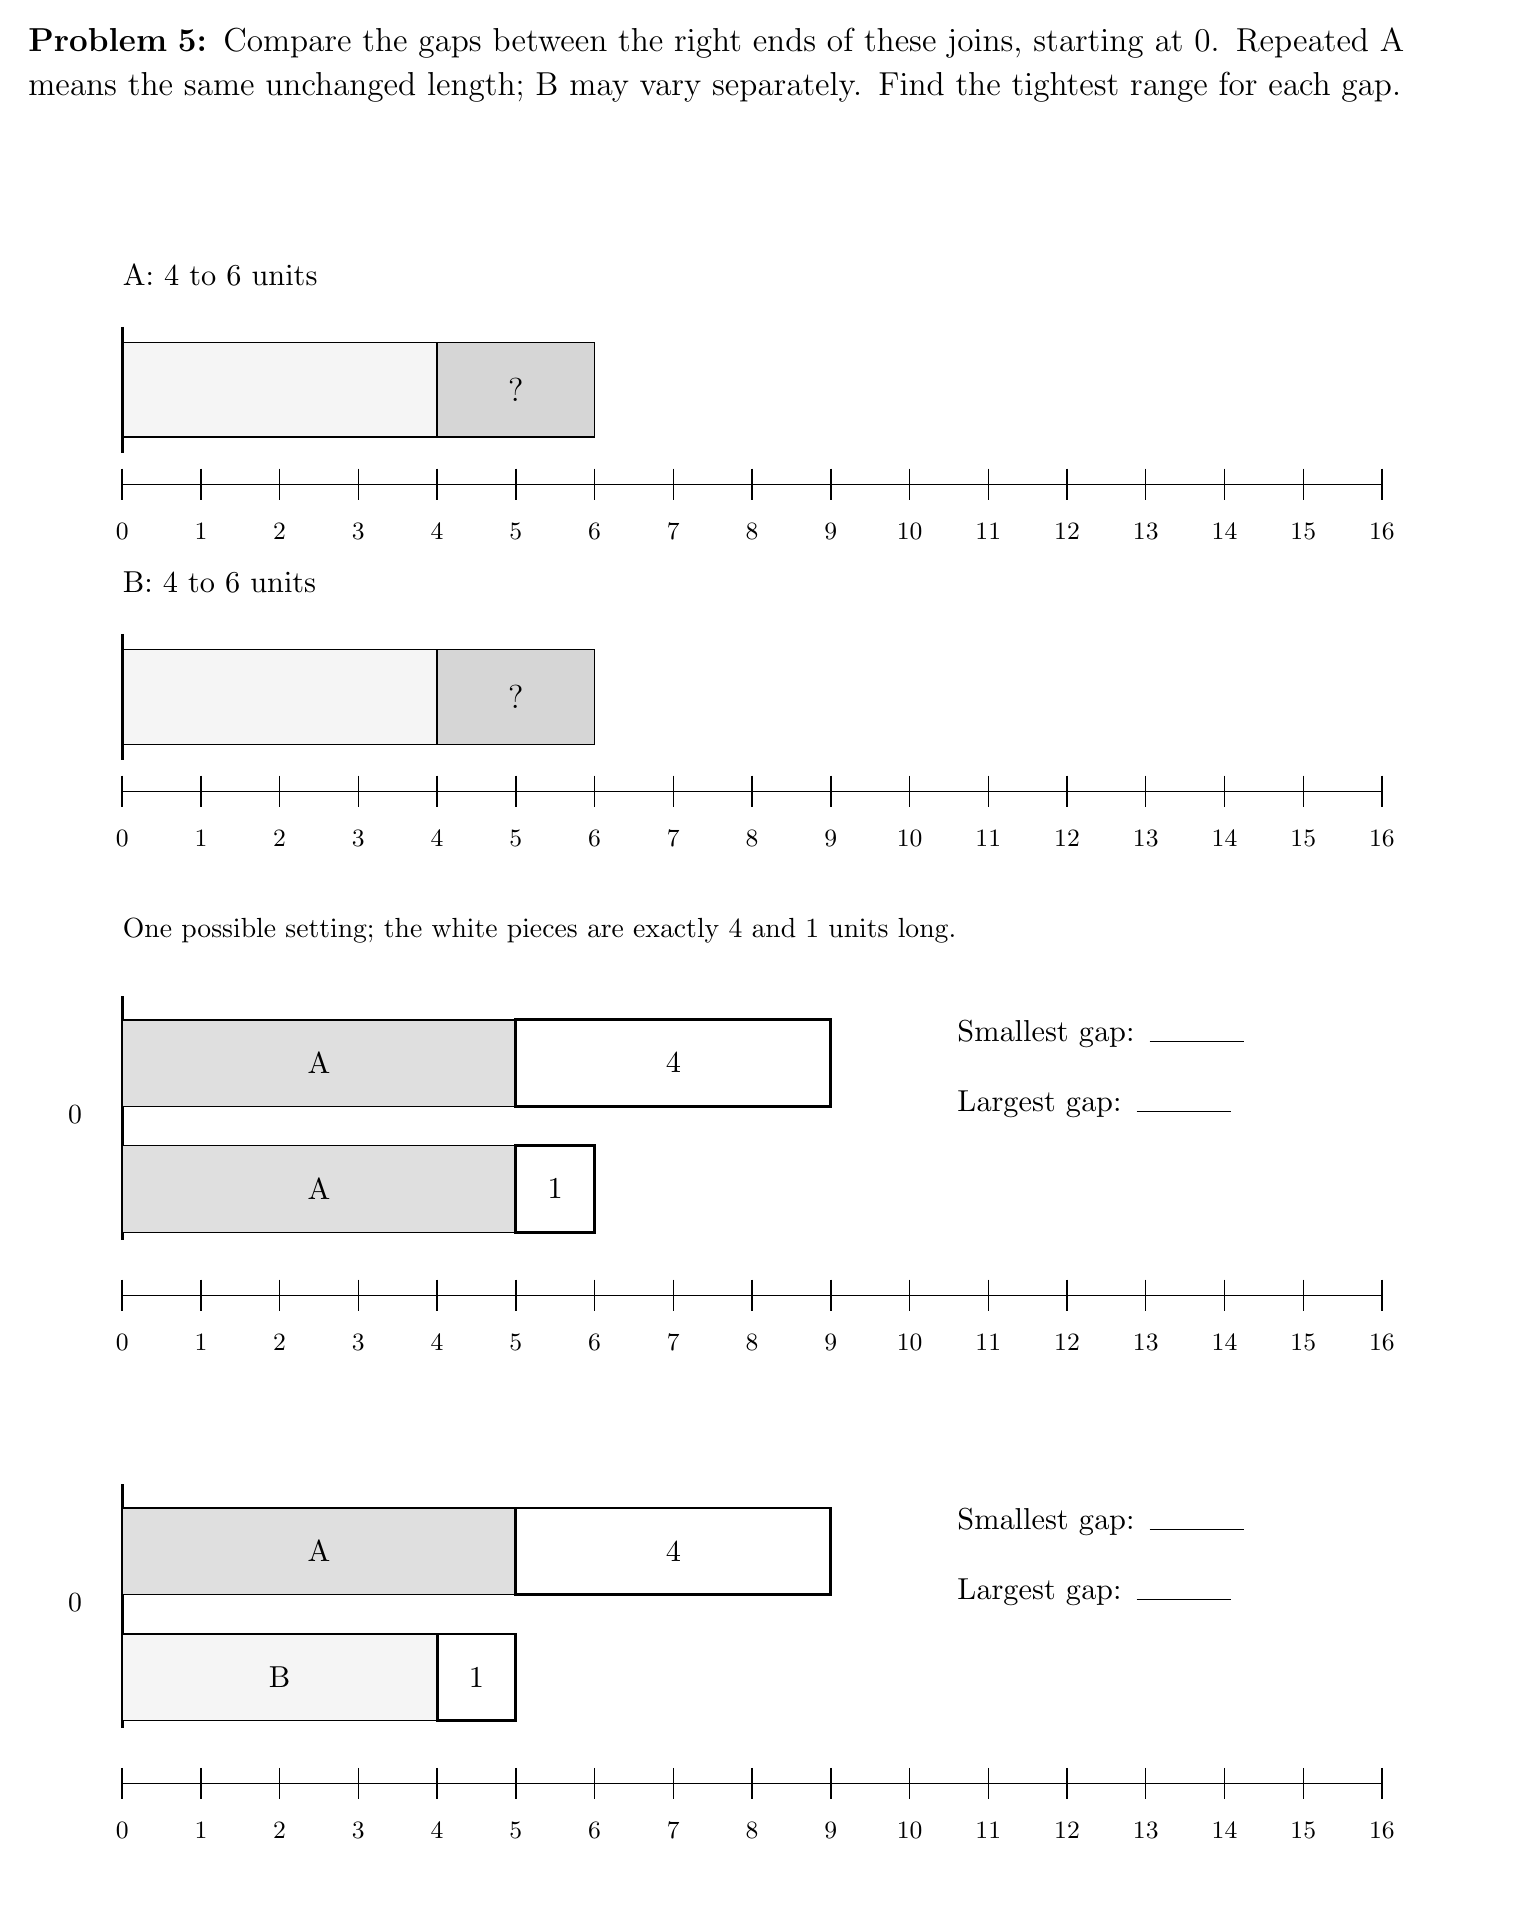
\begin{tikzpicture}[x=1mm,y=-1mm,line width=.5pt]
\path[use as bounding box] (0,0) rectangle (185,235);
\node[anchor=north west,inner sep=0pt,text width=180mm,font=\fontsize{13}{16}\selectfont] at (0,0) {\textbf{Problem 5:} Compare the gaps between the right ends of these joins, starting at 0. Repeated A means the same unchanged length; B may vary separately. Find the tightest range for each gap.};
\draw[fill=gray!8] (12,40) rectangle ++(40,12);
\draw[fill=gray!32] (52,40) rectangle ++(20,12);
\draw[line width=1.1pt] (12,38) -- (12,54);
\node[anchor=center,inner sep=1pt,font=\fontsize{12}{14}\selectfont] at (62.0,46.0) {?};
\node[anchor=north west,inner sep=0pt,text width=168mm,font=\fontsize{11}{14}\selectfont] at (12,30) {A: 4 to 6 units};
\draw[] (12,58) -- (172,58);
\draw[] (12,56) -- (12,60);
\node[anchor=center,inner sep=1pt,font=\fontsize{9}{11}\selectfont] at (12,64) {0};
\draw[] (22,56) -- (22,60);
\node[anchor=center,inner sep=1pt,font=\fontsize{9}{11}\selectfont] at (22,64) {1};
\draw[] (32,56) -- (32,60);
\node[anchor=center,inner sep=1pt,font=\fontsize{9}{11}\selectfont] at (32,64) {2};
\draw[] (42,56) -- (42,60);
\node[anchor=center,inner sep=1pt,font=\fontsize{9}{11}\selectfont] at (42,64) {3};
\draw[] (52,56) -- (52,60);
\node[anchor=center,inner sep=1pt,font=\fontsize{9}{11}\selectfont] at (52,64) {4};
\draw[] (62,56) -- (62,60);
\node[anchor=center,inner sep=1pt,font=\fontsize{9}{11}\selectfont] at (62,64) {5};
\draw[] (72,56) -- (72,60);
\node[anchor=center,inner sep=1pt,font=\fontsize{9}{11}\selectfont] at (72,64) {6};
\draw[] (82,56) -- (82,60);
\node[anchor=center,inner sep=1pt,font=\fontsize{9}{11}\selectfont] at (82,64) {7};
\draw[] (92,56) -- (92,60);
\node[anchor=center,inner sep=1pt,font=\fontsize{9}{11}\selectfont] at (92,64) {8};
\draw[] (102,56) -- (102,60);
\node[anchor=center,inner sep=1pt,font=\fontsize{9}{11}\selectfont] at (102,64) {9};
\draw[] (112,56) -- (112,60);
\node[anchor=center,inner sep=1pt,font=\fontsize{9}{11}\selectfont] at (112,64) {10};
\draw[] (122,56) -- (122,60);
\node[anchor=center,inner sep=1pt,font=\fontsize{9}{11}\selectfont] at (122,64) {11};
\draw[] (132,56) -- (132,60);
\node[anchor=center,inner sep=1pt,font=\fontsize{9}{11}\selectfont] at (132,64) {12};
\draw[] (142,56) -- (142,60);
\node[anchor=center,inner sep=1pt,font=\fontsize{9}{11}\selectfont] at (142,64) {13};
\draw[] (152,56) -- (152,60);
\node[anchor=center,inner sep=1pt,font=\fontsize{9}{11}\selectfont] at (152,64) {14};
\draw[] (162,56) -- (162,60);
\node[anchor=center,inner sep=1pt,font=\fontsize{9}{11}\selectfont] at (162,64) {15};
\draw[] (172,56) -- (172,60);
\node[anchor=center,inner sep=1pt,font=\fontsize{9}{11}\selectfont] at (172,64) {16};
\draw[fill=gray!8] (12,79) rectangle ++(40,12);
\draw[fill=gray!32] (52,79) rectangle ++(20,12);
\draw[line width=1.1pt] (12,77) -- (12,93);
\node[anchor=center,inner sep=1pt,font=\fontsize{12}{14}\selectfont] at (62.0,85.0) {?};
\node[anchor=north west,inner sep=0pt,text width=168mm,font=\fontsize{11}{14}\selectfont] at (12,69) {B: 4 to 6 units};
\draw[] (12,97) -- (172,97);
\draw[] (12,95) -- (12,99);
\node[anchor=center,inner sep=1pt,font=\fontsize{9}{11}\selectfont] at (12,103) {0};
\draw[] (22,95) -- (22,99);
\node[anchor=center,inner sep=1pt,font=\fontsize{9}{11}\selectfont] at (22,103) {1};
\draw[] (32,95) -- (32,99);
\node[anchor=center,inner sep=1pt,font=\fontsize{9}{11}\selectfont] at (32,103) {2};
\draw[] (42,95) -- (42,99);
\node[anchor=center,inner sep=1pt,font=\fontsize{9}{11}\selectfont] at (42,103) {3};
\draw[] (52,95) -- (52,99);
\node[anchor=center,inner sep=1pt,font=\fontsize{9}{11}\selectfont] at (52,103) {4};
\draw[] (62,95) -- (62,99);
\node[anchor=center,inner sep=1pt,font=\fontsize{9}{11}\selectfont] at (62,103) {5};
\draw[] (72,95) -- (72,99);
\node[anchor=center,inner sep=1pt,font=\fontsize{9}{11}\selectfont] at (72,103) {6};
\draw[] (82,95) -- (82,99);
\node[anchor=center,inner sep=1pt,font=\fontsize{9}{11}\selectfont] at (82,103) {7};
\draw[] (92,95) -- (92,99);
\node[anchor=center,inner sep=1pt,font=\fontsize{9}{11}\selectfont] at (92,103) {8};
\draw[] (102,95) -- (102,99);
\node[anchor=center,inner sep=1pt,font=\fontsize{9}{11}\selectfont] at (102,103) {9};
\draw[] (112,95) -- (112,99);
\node[anchor=center,inner sep=1pt,font=\fontsize{9}{11}\selectfont] at (112,103) {10};
\draw[] (122,95) -- (122,99);
\node[anchor=center,inner sep=1pt,font=\fontsize{9}{11}\selectfont] at (122,103) {11};
\draw[] (132,95) -- (132,99);
\node[anchor=center,inner sep=1pt,font=\fontsize{9}{11}\selectfont] at (132,103) {12};
\draw[] (142,95) -- (142,99);
\node[anchor=center,inner sep=1pt,font=\fontsize{9}{11}\selectfont] at (142,103) {13};
\draw[] (152,95) -- (152,99);
\node[anchor=center,inner sep=1pt,font=\fontsize{9}{11}\selectfont] at (152,103) {14};
\draw[] (162,95) -- (162,99);
\node[anchor=center,inner sep=1pt,font=\fontsize{9}{11}\selectfont] at (162,103) {15};
\draw[] (172,95) -- (172,99);
\node[anchor=center,inner sep=1pt,font=\fontsize{9}{11}\selectfont] at (172,103) {16};
\node[anchor=north west,inner sep=0pt,text width=180mm,font=\fontsize{10}{13}\selectfont] at (12,113) {One possible setting; the white pieces are exactly 4 and 1 units long.};
\draw[line width=1pt] (12,123) -- (12,154);
\draw[fill=gray!25] (12,126) rectangle ++(50,11);
\node[anchor=center,inner sep=1pt,font=\fontsize{11}{13}\selectfont] at (37.0,131.5) {A};
\draw[fill=white,line width=1pt] (62,126) rectangle ++(40,11);
\node[anchor=center,inner sep=1pt,font=\fontsize{11}{13}\selectfont] at (82,131.5) {4};
\draw[fill=gray!25] (12,142) rectangle ++(50,11);
\node[anchor=center,inner sep=1pt,font=\fontsize{11}{13}\selectfont] at (37.0,147.5) {A};
\draw[fill=white,line width=1pt] (62,142) rectangle ++(10,11);
\node[anchor=center,inner sep=1pt,font=\fontsize{11}{13}\selectfont] at (67,147.5) {1};
\node[anchor=center,inner sep=1pt,font=\fontsize{10}{12}\selectfont] at (6,138) {0};
\node[anchor=north west,inner sep=0pt,text width=65mm,font=\fontsize{11}{14}\selectfont] at (118,126) {Smallest gap: \rule{12mm}{.3pt}\\[4mm]Largest gap: \rule{12mm}{.3pt}};
\draw[] (12,161) -- (172,161);
\draw[] (12,159) -- (12,163);
\node[anchor=center,inner sep=1pt,font=\fontsize{9}{11}\selectfont] at (12,167) {0};
\draw[] (22,159) -- (22,163);
\node[anchor=center,inner sep=1pt,font=\fontsize{9}{11}\selectfont] at (22,167) {1};
\draw[] (32,159) -- (32,163);
\node[anchor=center,inner sep=1pt,font=\fontsize{9}{11}\selectfont] at (32,167) {2};
\draw[] (42,159) -- (42,163);
\node[anchor=center,inner sep=1pt,font=\fontsize{9}{11}\selectfont] at (42,167) {3};
\draw[] (52,159) -- (52,163);
\node[anchor=center,inner sep=1pt,font=\fontsize{9}{11}\selectfont] at (52,167) {4};
\draw[] (62,159) -- (62,163);
\node[anchor=center,inner sep=1pt,font=\fontsize{9}{11}\selectfont] at (62,167) {5};
\draw[] (72,159) -- (72,163);
\node[anchor=center,inner sep=1pt,font=\fontsize{9}{11}\selectfont] at (72,167) {6};
\draw[] (82,159) -- (82,163);
\node[anchor=center,inner sep=1pt,font=\fontsize{9}{11}\selectfont] at (82,167) {7};
\draw[] (92,159) -- (92,163);
\node[anchor=center,inner sep=1pt,font=\fontsize{9}{11}\selectfont] at (92,167) {8};
\draw[] (102,159) -- (102,163);
\node[anchor=center,inner sep=1pt,font=\fontsize{9}{11}\selectfont] at (102,167) {9};
\draw[] (112,159) -- (112,163);
\node[anchor=center,inner sep=1pt,font=\fontsize{9}{11}\selectfont] at (112,167) {10};
\draw[] (122,159) -- (122,163);
\node[anchor=center,inner sep=1pt,font=\fontsize{9}{11}\selectfont] at (122,167) {11};
\draw[] (132,159) -- (132,163);
\node[anchor=center,inner sep=1pt,font=\fontsize{9}{11}\selectfont] at (132,167) {12};
\draw[] (142,159) -- (142,163);
\node[anchor=center,inner sep=1pt,font=\fontsize{9}{11}\selectfont] at (142,167) {13};
\draw[] (152,159) -- (152,163);
\node[anchor=center,inner sep=1pt,font=\fontsize{9}{11}\selectfont] at (152,167) {14};
\draw[] (162,159) -- (162,163);
\node[anchor=center,inner sep=1pt,font=\fontsize{9}{11}\selectfont] at (162,167) {15};
\draw[] (172,159) -- (172,163);
\node[anchor=center,inner sep=1pt,font=\fontsize{9}{11}\selectfont] at (172,167) {16};
\draw[line width=1pt] (12,185) -- (12,216);
\draw[fill=gray!25] (12,188) rectangle ++(50,11);
\node[anchor=center,inner sep=1pt,font=\fontsize{11}{13}\selectfont] at (37.0,193.5) {A};
\draw[fill=white,line width=1pt] (62,188) rectangle ++(40,11);
\node[anchor=center,inner sep=1pt,font=\fontsize{11}{13}\selectfont] at (82,193.5) {4};
\draw[fill=gray!8] (12,204) rectangle ++(40,11);
\node[anchor=center,inner sep=1pt,font=\fontsize{11}{13}\selectfont] at (32.0,209.5) {B};
\draw[fill=white,line width=1pt] (52,204) rectangle ++(10,11);
\node[anchor=center,inner sep=1pt,font=\fontsize{11}{13}\selectfont] at (57,209.5) {1};
\node[anchor=center,inner sep=1pt,font=\fontsize{10}{12}\selectfont] at (6,200) {0};
\node[anchor=north west,inner sep=0pt,text width=65mm,font=\fontsize{11}{14}\selectfont] at (118,188) {Smallest gap: \rule{12mm}{.3pt}\\[4mm]Largest gap: \rule{12mm}{.3pt}};
\draw[] (12,223) -- (172,223);
\draw[] (12,221) -- (12,225);
\node[anchor=center,inner sep=1pt,font=\fontsize{9}{11}\selectfont] at (12,229) {0};
\draw[] (22,221) -- (22,225);
\node[anchor=center,inner sep=1pt,font=\fontsize{9}{11}\selectfont] at (22,229) {1};
\draw[] (32,221) -- (32,225);
\node[anchor=center,inner sep=1pt,font=\fontsize{9}{11}\selectfont] at (32,229) {2};
\draw[] (42,221) -- (42,225);
\node[anchor=center,inner sep=1pt,font=\fontsize{9}{11}\selectfont] at (42,229) {3};
\draw[] (52,221) -- (52,225);
\node[anchor=center,inner sep=1pt,font=\fontsize{9}{11}\selectfont] at (52,229) {4};
\draw[] (62,221) -- (62,225);
\node[anchor=center,inner sep=1pt,font=\fontsize{9}{11}\selectfont] at (62,229) {5};
\draw[] (72,221) -- (72,225);
\node[anchor=center,inner sep=1pt,font=\fontsize{9}{11}\selectfont] at (72,229) {6};
\draw[] (82,221) -- (82,225);
\node[anchor=center,inner sep=1pt,font=\fontsize{9}{11}\selectfont] at (82,229) {7};
\draw[] (92,221) -- (92,225);
\node[anchor=center,inner sep=1pt,font=\fontsize{9}{11}\selectfont] at (92,229) {8};
\draw[] (102,221) -- (102,225);
\node[anchor=center,inner sep=1pt,font=\fontsize{9}{11}\selectfont] at (102,229) {9};
\draw[] (112,221) -- (112,225);
\node[anchor=center,inner sep=1pt,font=\fontsize{9}{11}\selectfont] at (112,229) {10};
\draw[] (122,221) -- (122,225);
\node[anchor=center,inner sep=1pt,font=\fontsize{9}{11}\selectfont] at (122,229) {11};
\draw[] (132,221) -- (132,225);
\node[anchor=center,inner sep=1pt,font=\fontsize{9}{11}\selectfont] at (132,229) {12};
\draw[] (142,221) -- (142,225);
\node[anchor=center,inner sep=1pt,font=\fontsize{9}{11}\selectfont] at (142,229) {13};
\draw[] (152,221) -- (152,225);
\node[anchor=center,inner sep=1pt,font=\fontsize{9}{11}\selectfont] at (152,229) {14};
\draw[] (162,221) -- (162,225);
\node[anchor=center,inner sep=1pt,font=\fontsize{9}{11}\selectfont] at (162,229) {15};
\draw[] (172,221) -- (172,225);
\node[anchor=center,inner sep=1pt,font=\fontsize{9}{11}\selectfont] at (172,229) {16};
\end{tikzpicture}
\newpage
\noindent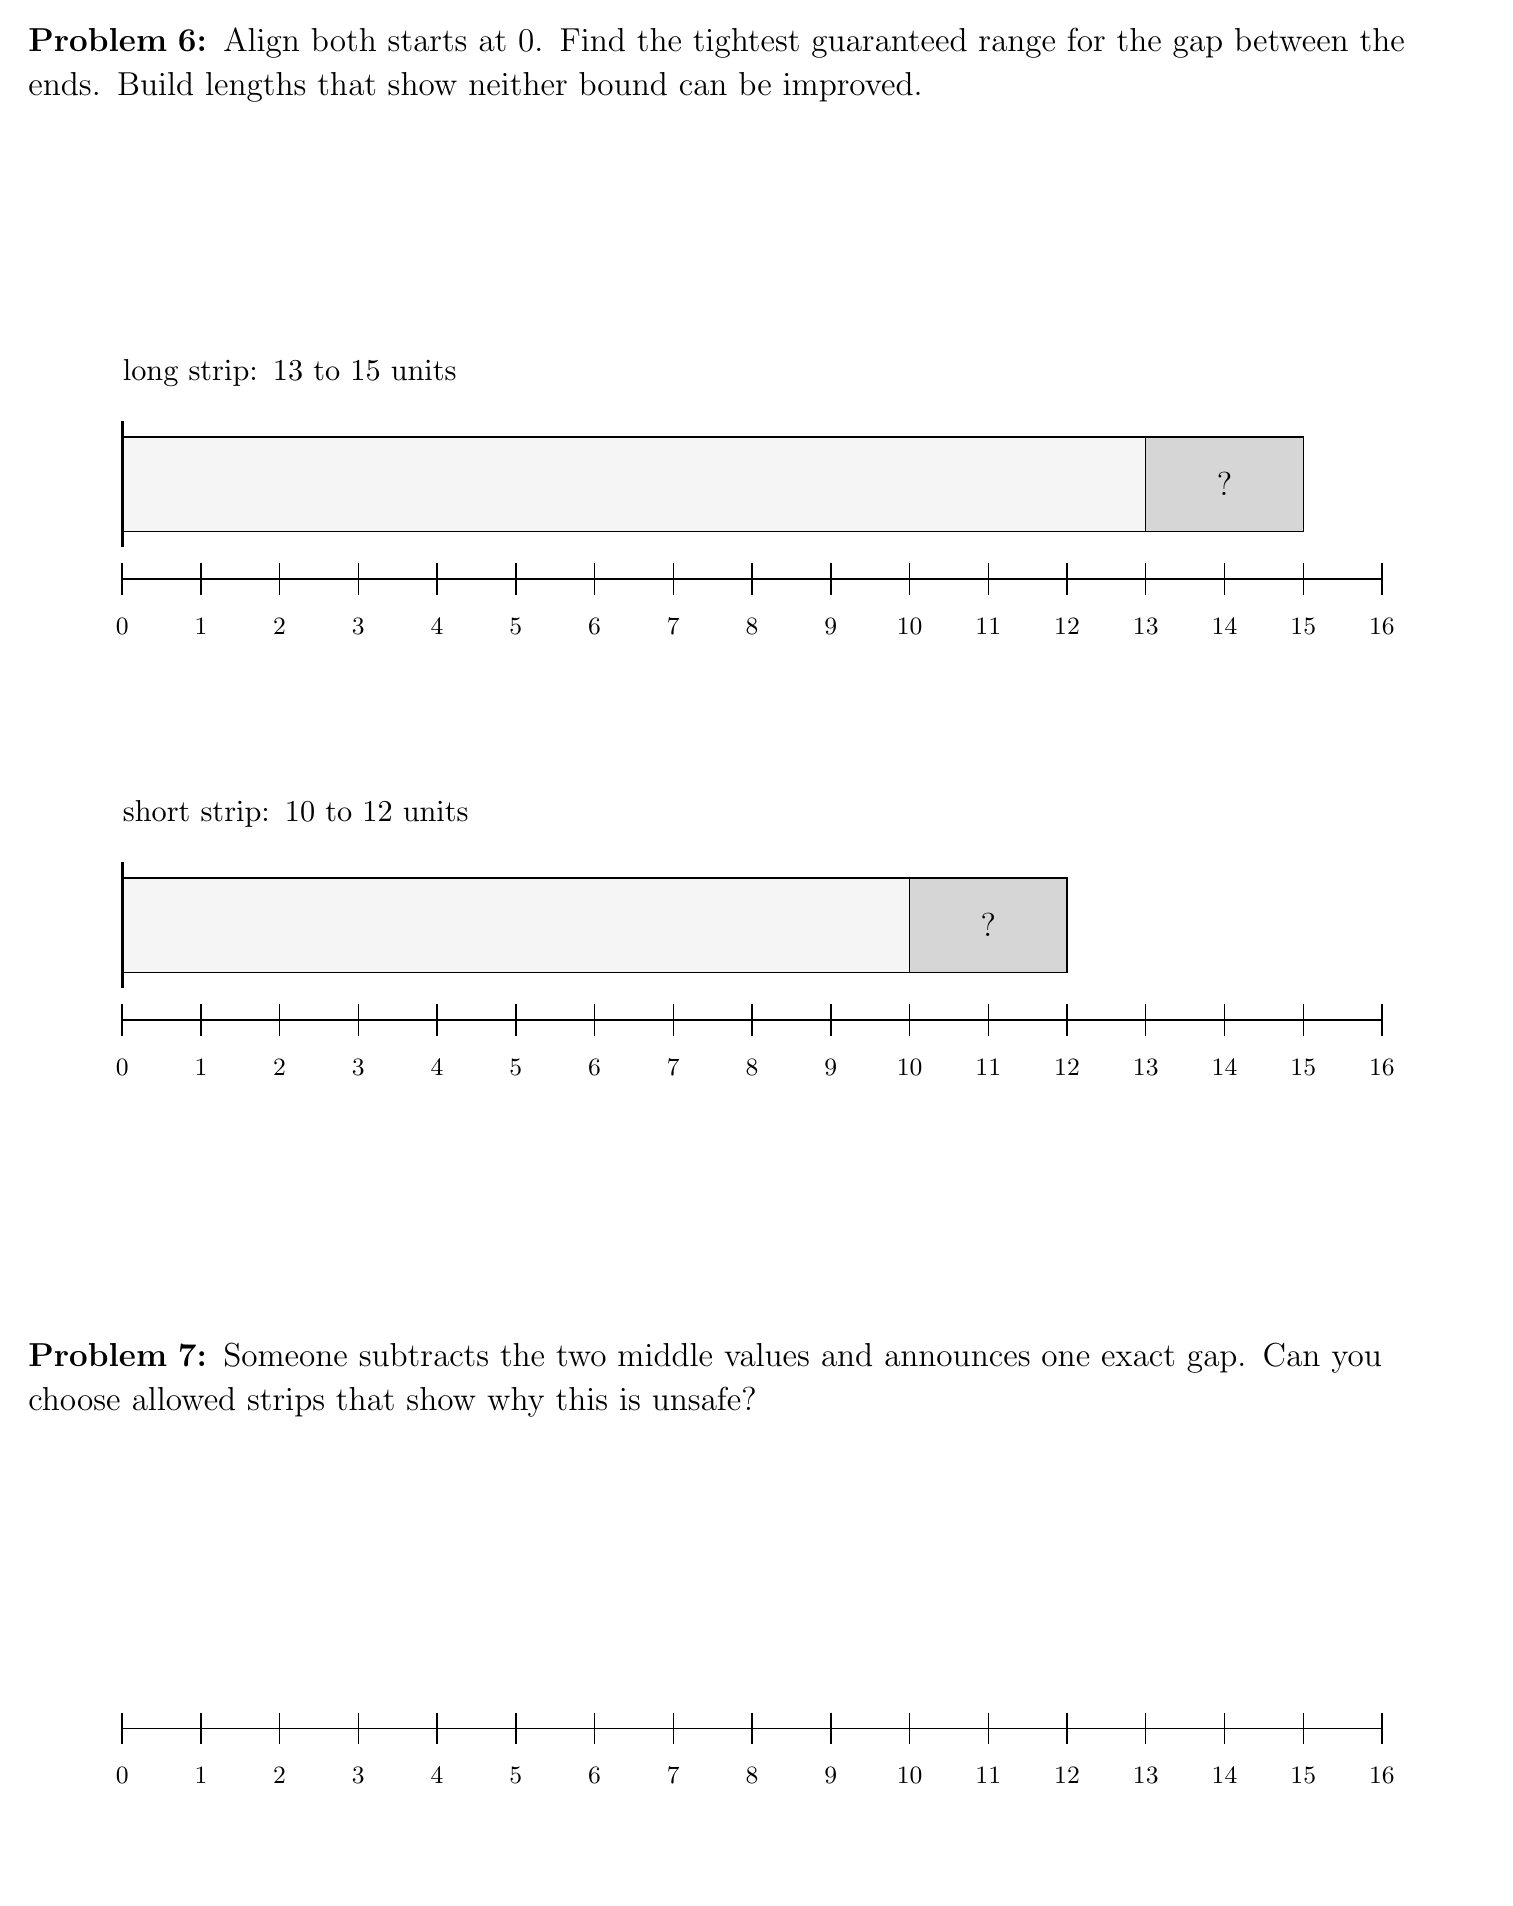
\begin{tikzpicture}[x=1mm,y=-1mm,line width=.5pt]
\path[use as bounding box] (0,0) rectangle (185,235);
\node[anchor=north west,inner sep=0pt,text width=180mm,font=\fontsize{13}{16}\selectfont] at (0,0) {\textbf{Problem 6:} Align both starts at 0. Find the tightest guaranteed range for the gap between the ends. Build lengths that show neither bound can be improved.};
\draw[fill=gray!8] (12,52) rectangle ++(130,12);
\draw[fill=gray!32] (142,52) rectangle ++(20,12);
\draw[line width=1.1pt] (12,50) -- (12,66);
\node[anchor=center,inner sep=1pt,font=\fontsize{12}{14}\selectfont] at (152.0,58.0) {?};
\node[anchor=north west,inner sep=0pt,text width=168mm,font=\fontsize{11}{14}\selectfont] at (12,42) {long strip: 13 to 15 units};
\draw[] (12,70) -- (172,70);
\draw[] (12,68) -- (12,72);
\node[anchor=center,inner sep=1pt,font=\fontsize{9}{11}\selectfont] at (12,76) {0};
\draw[] (22,68) -- (22,72);
\node[anchor=center,inner sep=1pt,font=\fontsize{9}{11}\selectfont] at (22,76) {1};
\draw[] (32,68) -- (32,72);
\node[anchor=center,inner sep=1pt,font=\fontsize{9}{11}\selectfont] at (32,76) {2};
\draw[] (42,68) -- (42,72);
\node[anchor=center,inner sep=1pt,font=\fontsize{9}{11}\selectfont] at (42,76) {3};
\draw[] (52,68) -- (52,72);
\node[anchor=center,inner sep=1pt,font=\fontsize{9}{11}\selectfont] at (52,76) {4};
\draw[] (62,68) -- (62,72);
\node[anchor=center,inner sep=1pt,font=\fontsize{9}{11}\selectfont] at (62,76) {5};
\draw[] (72,68) -- (72,72);
\node[anchor=center,inner sep=1pt,font=\fontsize{9}{11}\selectfont] at (72,76) {6};
\draw[] (82,68) -- (82,72);
\node[anchor=center,inner sep=1pt,font=\fontsize{9}{11}\selectfont] at (82,76) {7};
\draw[] (92,68) -- (92,72);
\node[anchor=center,inner sep=1pt,font=\fontsize{9}{11}\selectfont] at (92,76) {8};
\draw[] (102,68) -- (102,72);
\node[anchor=center,inner sep=1pt,font=\fontsize{9}{11}\selectfont] at (102,76) {9};
\draw[] (112,68) -- (112,72);
\node[anchor=center,inner sep=1pt,font=\fontsize{9}{11}\selectfont] at (112,76) {10};
\draw[] (122,68) -- (122,72);
\node[anchor=center,inner sep=1pt,font=\fontsize{9}{11}\selectfont] at (122,76) {11};
\draw[] (132,68) -- (132,72);
\node[anchor=center,inner sep=1pt,font=\fontsize{9}{11}\selectfont] at (132,76) {12};
\draw[] (142,68) -- (142,72);
\node[anchor=center,inner sep=1pt,font=\fontsize{9}{11}\selectfont] at (142,76) {13};
\draw[] (152,68) -- (152,72);
\node[anchor=center,inner sep=1pt,font=\fontsize{9}{11}\selectfont] at (152,76) {14};
\draw[] (162,68) -- (162,72);
\node[anchor=center,inner sep=1pt,font=\fontsize{9}{11}\selectfont] at (162,76) {15};
\draw[] (172,68) -- (172,72);
\node[anchor=center,inner sep=1pt,font=\fontsize{9}{11}\selectfont] at (172,76) {16};
\draw[fill=gray!8] (12,108) rectangle ++(100,12);
\draw[fill=gray!32] (112,108) rectangle ++(20,12);
\draw[line width=1.1pt] (12,106) -- (12,122);
\node[anchor=center,inner sep=1pt,font=\fontsize{12}{14}\selectfont] at (122.0,114.0) {?};
\node[anchor=north west,inner sep=0pt,text width=168mm,font=\fontsize{11}{14}\selectfont] at (12,98) {short strip: 10 to 12 units};
\draw[] (12,126) -- (172,126);
\draw[] (12,124) -- (12,128);
\node[anchor=center,inner sep=1pt,font=\fontsize{9}{11}\selectfont] at (12,132) {0};
\draw[] (22,124) -- (22,128);
\node[anchor=center,inner sep=1pt,font=\fontsize{9}{11}\selectfont] at (22,132) {1};
\draw[] (32,124) -- (32,128);
\node[anchor=center,inner sep=1pt,font=\fontsize{9}{11}\selectfont] at (32,132) {2};
\draw[] (42,124) -- (42,128);
\node[anchor=center,inner sep=1pt,font=\fontsize{9}{11}\selectfont] at (42,132) {3};
\draw[] (52,124) -- (52,128);
\node[anchor=center,inner sep=1pt,font=\fontsize{9}{11}\selectfont] at (52,132) {4};
\draw[] (62,124) -- (62,128);
\node[anchor=center,inner sep=1pt,font=\fontsize{9}{11}\selectfont] at (62,132) {5};
\draw[] (72,124) -- (72,128);
\node[anchor=center,inner sep=1pt,font=\fontsize{9}{11}\selectfont] at (72,132) {6};
\draw[] (82,124) -- (82,128);
\node[anchor=center,inner sep=1pt,font=\fontsize{9}{11}\selectfont] at (82,132) {7};
\draw[] (92,124) -- (92,128);
\node[anchor=center,inner sep=1pt,font=\fontsize{9}{11}\selectfont] at (92,132) {8};
\draw[] (102,124) -- (102,128);
\node[anchor=center,inner sep=1pt,font=\fontsize{9}{11}\selectfont] at (102,132) {9};
\draw[] (112,124) -- (112,128);
\node[anchor=center,inner sep=1pt,font=\fontsize{9}{11}\selectfont] at (112,132) {10};
\draw[] (122,124) -- (122,128);
\node[anchor=center,inner sep=1pt,font=\fontsize{9}{11}\selectfont] at (122,132) {11};
\draw[] (132,124) -- (132,128);
\node[anchor=center,inner sep=1pt,font=\fontsize{9}{11}\selectfont] at (132,132) {12};
\draw[] (142,124) -- (142,128);
\node[anchor=center,inner sep=1pt,font=\fontsize{9}{11}\selectfont] at (142,132) {13};
\draw[] (152,124) -- (152,128);
\node[anchor=center,inner sep=1pt,font=\fontsize{9}{11}\selectfont] at (152,132) {14};
\draw[] (162,124) -- (162,128);
\node[anchor=center,inner sep=1pt,font=\fontsize{9}{11}\selectfont] at (162,132) {15};
\draw[] (172,124) -- (172,128);
\node[anchor=center,inner sep=1pt,font=\fontsize{9}{11}\selectfont] at (172,132) {16};
\node[anchor=north west,inner sep=0pt,text width=180mm,font=\fontsize{13}{16}\selectfont] at (0,167) {\textbf{Problem 7:} Someone subtracts the two middle values and announces one exact gap. Can you choose allowed strips that show why this is unsafe?};
\draw[] (12,216) -- (172,216);
\draw[] (12,214) -- (12,218);
\node[anchor=center,inner sep=1pt,font=\fontsize{9}{11}\selectfont] at (12,222) {0};
\draw[] (22,214) -- (22,218);
\node[anchor=center,inner sep=1pt,font=\fontsize{9}{11}\selectfont] at (22,222) {1};
\draw[] (32,214) -- (32,218);
\node[anchor=center,inner sep=1pt,font=\fontsize{9}{11}\selectfont] at (32,222) {2};
\draw[] (42,214) -- (42,218);
\node[anchor=center,inner sep=1pt,font=\fontsize{9}{11}\selectfont] at (42,222) {3};
\draw[] (52,214) -- (52,218);
\node[anchor=center,inner sep=1pt,font=\fontsize{9}{11}\selectfont] at (52,222) {4};
\draw[] (62,214) -- (62,218);
\node[anchor=center,inner sep=1pt,font=\fontsize{9}{11}\selectfont] at (62,222) {5};
\draw[] (72,214) -- (72,218);
\node[anchor=center,inner sep=1pt,font=\fontsize{9}{11}\selectfont] at (72,222) {6};
\draw[] (82,214) -- (82,218);
\node[anchor=center,inner sep=1pt,font=\fontsize{9}{11}\selectfont] at (82,222) {7};
\draw[] (92,214) -- (92,218);
\node[anchor=center,inner sep=1pt,font=\fontsize{9}{11}\selectfont] at (92,222) {8};
\draw[] (102,214) -- (102,218);
\node[anchor=center,inner sep=1pt,font=\fontsize{9}{11}\selectfont] at (102,222) {9};
\draw[] (112,214) -- (112,218);
\node[anchor=center,inner sep=1pt,font=\fontsize{9}{11}\selectfont] at (112,222) {10};
\draw[] (122,214) -- (122,218);
\node[anchor=center,inner sep=1pt,font=\fontsize{9}{11}\selectfont] at (122,222) {11};
\draw[] (132,214) -- (132,218);
\node[anchor=center,inner sep=1pt,font=\fontsize{9}{11}\selectfont] at (132,222) {12};
\draw[] (142,214) -- (142,218);
\node[anchor=center,inner sep=1pt,font=\fontsize{9}{11}\selectfont] at (142,222) {13};
\draw[] (152,214) -- (152,218);
\node[anchor=center,inner sep=1pt,font=\fontsize{9}{11}\selectfont] at (152,222) {14};
\draw[] (162,214) -- (162,218);
\node[anchor=center,inner sep=1pt,font=\fontsize{9}{11}\selectfont] at (162,222) {15};
\draw[] (172,214) -- (172,218);
\node[anchor=center,inner sep=1pt,font=\fontsize{9}{11}\selectfont] at (172,222) {16};
\end{tikzpicture}
\newpage
\noindent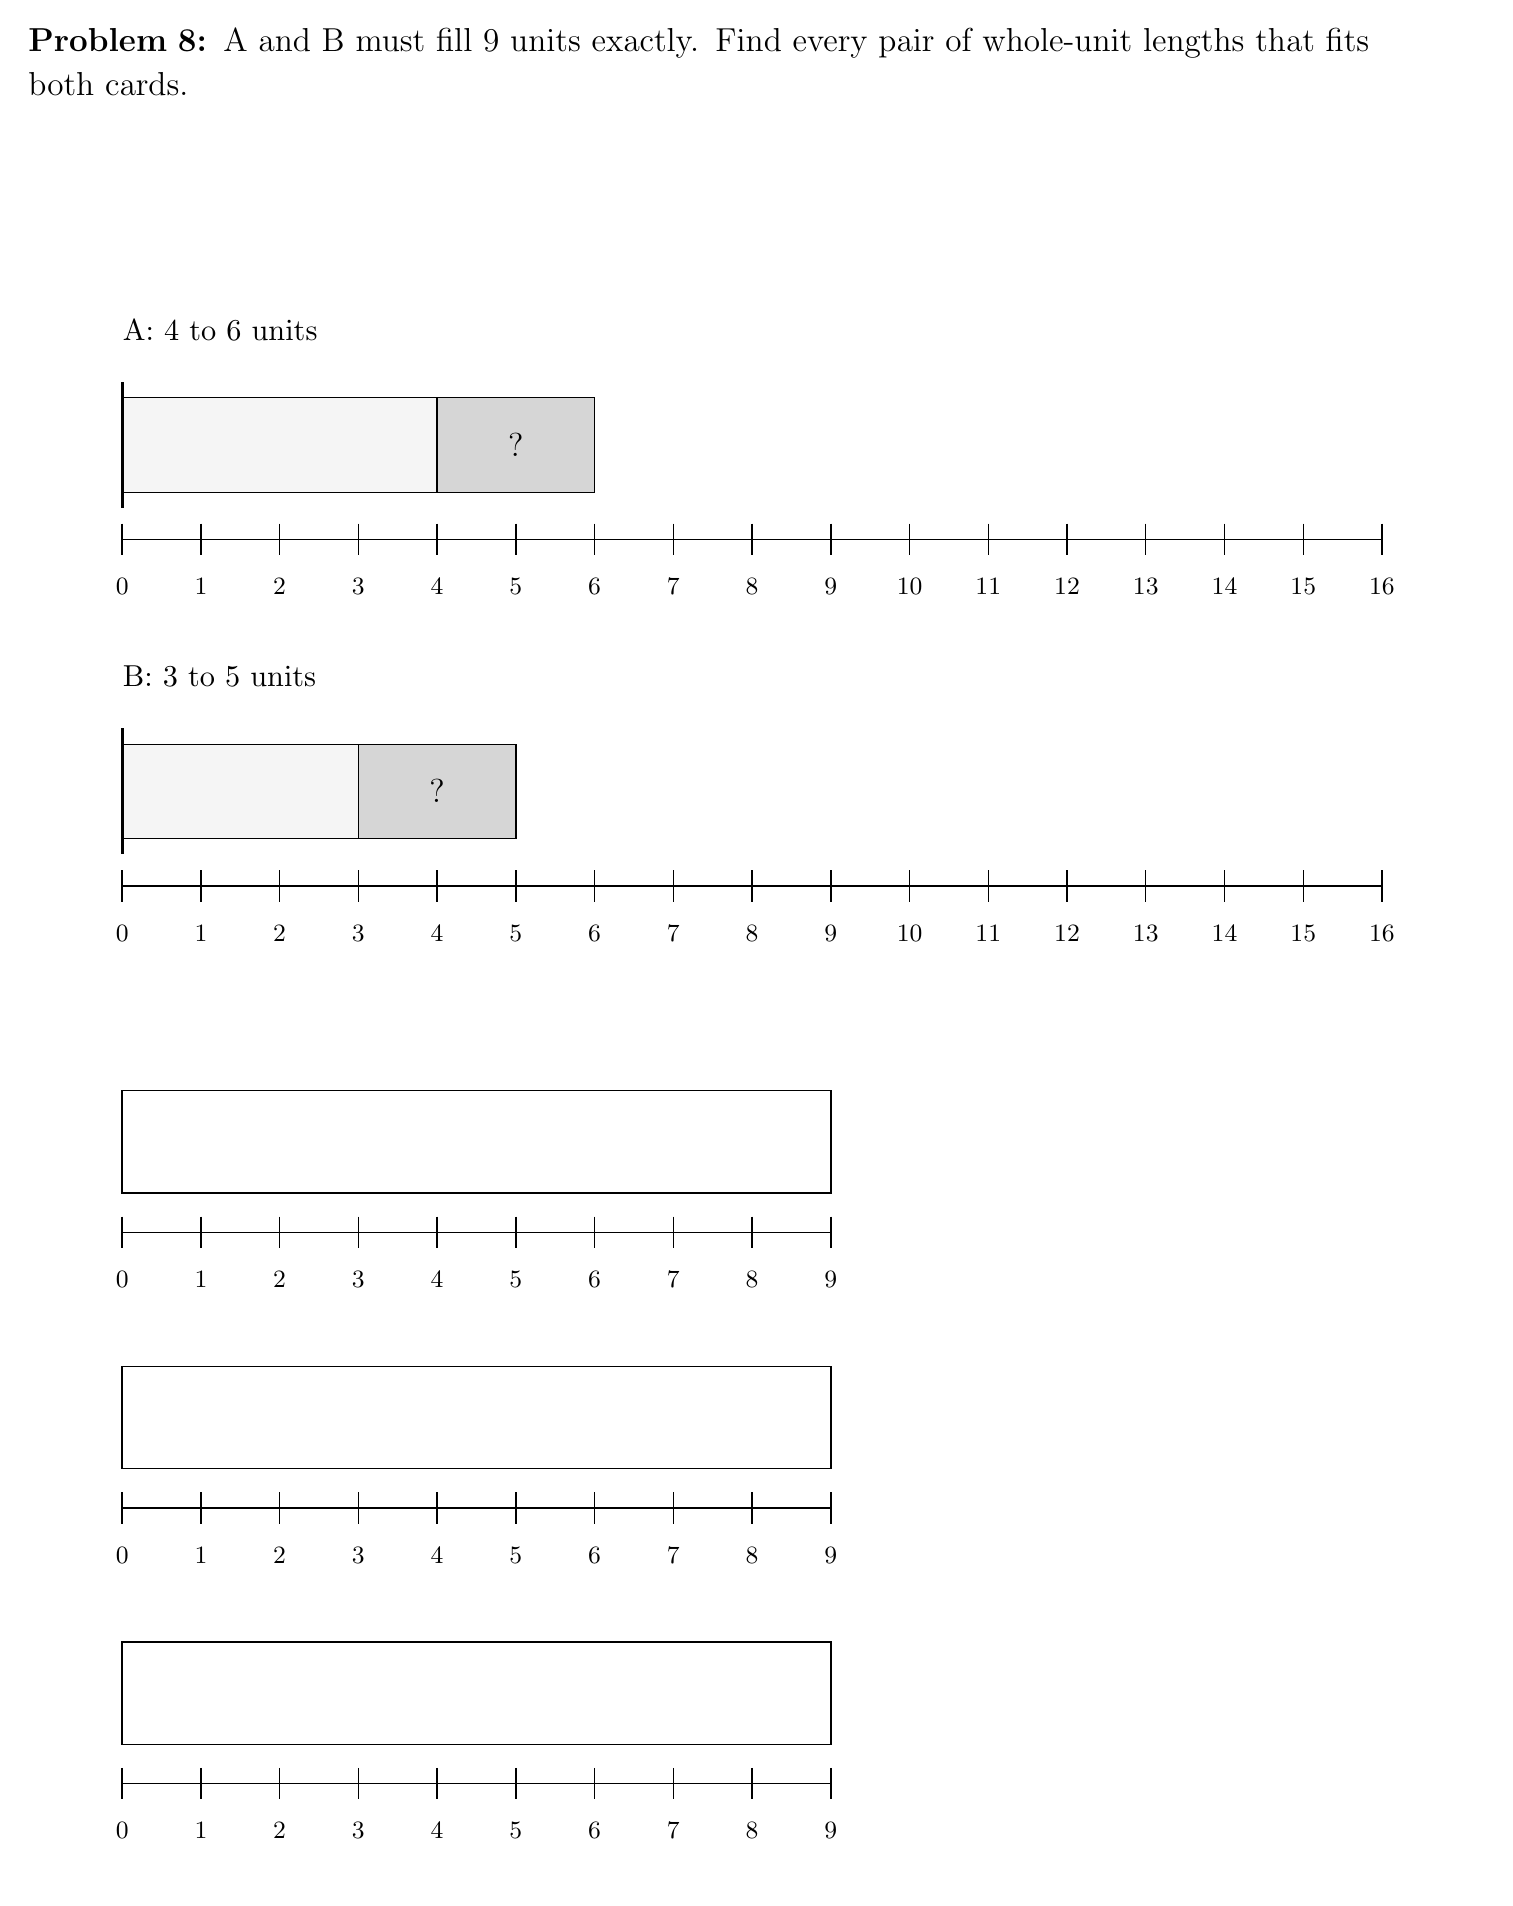
\begin{tikzpicture}[x=1mm,y=-1mm,line width=.5pt]
\path[use as bounding box] (0,0) rectangle (185,235);
\node[anchor=north west,inner sep=0pt,text width=180mm,font=\fontsize{13}{16}\selectfont] at (0,0) {\textbf{Problem 8:} A and B must fill 9 units exactly. Find every pair of whole-unit lengths that fits both cards.};
\draw[fill=gray!8] (12,47) rectangle ++(40,12);
\draw[fill=gray!32] (52,47) rectangle ++(20,12);
\draw[line width=1.1pt] (12,45) -- (12,61);
\node[anchor=center,inner sep=1pt,font=\fontsize{12}{14}\selectfont] at (62.0,53.0) {?};
\node[anchor=north west,inner sep=0pt,text width=168mm,font=\fontsize{11}{14}\selectfont] at (12,37) {A: 4 to 6 units};
\draw[] (12,65) -- (172,65);
\draw[] (12,63) -- (12,67);
\node[anchor=center,inner sep=1pt,font=\fontsize{9}{11}\selectfont] at (12,71) {0};
\draw[] (22,63) -- (22,67);
\node[anchor=center,inner sep=1pt,font=\fontsize{9}{11}\selectfont] at (22,71) {1};
\draw[] (32,63) -- (32,67);
\node[anchor=center,inner sep=1pt,font=\fontsize{9}{11}\selectfont] at (32,71) {2};
\draw[] (42,63) -- (42,67);
\node[anchor=center,inner sep=1pt,font=\fontsize{9}{11}\selectfont] at (42,71) {3};
\draw[] (52,63) -- (52,67);
\node[anchor=center,inner sep=1pt,font=\fontsize{9}{11}\selectfont] at (52,71) {4};
\draw[] (62,63) -- (62,67);
\node[anchor=center,inner sep=1pt,font=\fontsize{9}{11}\selectfont] at (62,71) {5};
\draw[] (72,63) -- (72,67);
\node[anchor=center,inner sep=1pt,font=\fontsize{9}{11}\selectfont] at (72,71) {6};
\draw[] (82,63) -- (82,67);
\node[anchor=center,inner sep=1pt,font=\fontsize{9}{11}\selectfont] at (82,71) {7};
\draw[] (92,63) -- (92,67);
\node[anchor=center,inner sep=1pt,font=\fontsize{9}{11}\selectfont] at (92,71) {8};
\draw[] (102,63) -- (102,67);
\node[anchor=center,inner sep=1pt,font=\fontsize{9}{11}\selectfont] at (102,71) {9};
\draw[] (112,63) -- (112,67);
\node[anchor=center,inner sep=1pt,font=\fontsize{9}{11}\selectfont] at (112,71) {10};
\draw[] (122,63) -- (122,67);
\node[anchor=center,inner sep=1pt,font=\fontsize{9}{11}\selectfont] at (122,71) {11};
\draw[] (132,63) -- (132,67);
\node[anchor=center,inner sep=1pt,font=\fontsize{9}{11}\selectfont] at (132,71) {12};
\draw[] (142,63) -- (142,67);
\node[anchor=center,inner sep=1pt,font=\fontsize{9}{11}\selectfont] at (142,71) {13};
\draw[] (152,63) -- (152,67);
\node[anchor=center,inner sep=1pt,font=\fontsize{9}{11}\selectfont] at (152,71) {14};
\draw[] (162,63) -- (162,67);
\node[anchor=center,inner sep=1pt,font=\fontsize{9}{11}\selectfont] at (162,71) {15};
\draw[] (172,63) -- (172,67);
\node[anchor=center,inner sep=1pt,font=\fontsize{9}{11}\selectfont] at (172,71) {16};
\draw[fill=gray!8] (12,91) rectangle ++(30,12);
\draw[fill=gray!32] (42,91) rectangle ++(20,12);
\draw[line width=1.1pt] (12,89) -- (12,105);
\node[anchor=center,inner sep=1pt,font=\fontsize{12}{14}\selectfont] at (52.0,97.0) {?};
\node[anchor=north west,inner sep=0pt,text width=168mm,font=\fontsize{11}{14}\selectfont] at (12,81) {B: 3 to 5 units};
\draw[] (12,109) -- (172,109);
\draw[] (12,107) -- (12,111);
\node[anchor=center,inner sep=1pt,font=\fontsize{9}{11}\selectfont] at (12,115) {0};
\draw[] (22,107) -- (22,111);
\node[anchor=center,inner sep=1pt,font=\fontsize{9}{11}\selectfont] at (22,115) {1};
\draw[] (32,107) -- (32,111);
\node[anchor=center,inner sep=1pt,font=\fontsize{9}{11}\selectfont] at (32,115) {2};
\draw[] (42,107) -- (42,111);
\node[anchor=center,inner sep=1pt,font=\fontsize{9}{11}\selectfont] at (42,115) {3};
\draw[] (52,107) -- (52,111);
\node[anchor=center,inner sep=1pt,font=\fontsize{9}{11}\selectfont] at (52,115) {4};
\draw[] (62,107) -- (62,111);
\node[anchor=center,inner sep=1pt,font=\fontsize{9}{11}\selectfont] at (62,115) {5};
\draw[] (72,107) -- (72,111);
\node[anchor=center,inner sep=1pt,font=\fontsize{9}{11}\selectfont] at (72,115) {6};
\draw[] (82,107) -- (82,111);
\node[anchor=center,inner sep=1pt,font=\fontsize{9}{11}\selectfont] at (82,115) {7};
\draw[] (92,107) -- (92,111);
\node[anchor=center,inner sep=1pt,font=\fontsize{9}{11}\selectfont] at (92,115) {8};
\draw[] (102,107) -- (102,111);
\node[anchor=center,inner sep=1pt,font=\fontsize{9}{11}\selectfont] at (102,115) {9};
\draw[] (112,107) -- (112,111);
\node[anchor=center,inner sep=1pt,font=\fontsize{9}{11}\selectfont] at (112,115) {10};
\draw[] (122,107) -- (122,111);
\node[anchor=center,inner sep=1pt,font=\fontsize{9}{11}\selectfont] at (122,115) {11};
\draw[] (132,107) -- (132,111);
\node[anchor=center,inner sep=1pt,font=\fontsize{9}{11}\selectfont] at (132,115) {12};
\draw[] (142,107) -- (142,111);
\node[anchor=center,inner sep=1pt,font=\fontsize{9}{11}\selectfont] at (142,115) {13};
\draw[] (152,107) -- (152,111);
\node[anchor=center,inner sep=1pt,font=\fontsize{9}{11}\selectfont] at (152,115) {14};
\draw[] (162,107) -- (162,111);
\node[anchor=center,inner sep=1pt,font=\fontsize{9}{11}\selectfont] at (162,115) {15};
\draw[] (172,107) -- (172,111);
\node[anchor=center,inner sep=1pt,font=\fontsize{9}{11}\selectfont] at (172,115) {16};
\draw[] (12,135) rectangle ++(90,13);
\draw[] (12,153) -- (102,153);
\draw[] (12,151) -- (12,155);
\node[anchor=center,inner sep=1pt,font=\fontsize{9}{11}\selectfont] at (12,159) {0};
\draw[] (22,151) -- (22,155);
\node[anchor=center,inner sep=1pt,font=\fontsize{9}{11}\selectfont] at (22,159) {1};
\draw[] (32,151) -- (32,155);
\node[anchor=center,inner sep=1pt,font=\fontsize{9}{11}\selectfont] at (32,159) {2};
\draw[] (42,151) -- (42,155);
\node[anchor=center,inner sep=1pt,font=\fontsize{9}{11}\selectfont] at (42,159) {3};
\draw[] (52,151) -- (52,155);
\node[anchor=center,inner sep=1pt,font=\fontsize{9}{11}\selectfont] at (52,159) {4};
\draw[] (62,151) -- (62,155);
\node[anchor=center,inner sep=1pt,font=\fontsize{9}{11}\selectfont] at (62,159) {5};
\draw[] (72,151) -- (72,155);
\node[anchor=center,inner sep=1pt,font=\fontsize{9}{11}\selectfont] at (72,159) {6};
\draw[] (82,151) -- (82,155);
\node[anchor=center,inner sep=1pt,font=\fontsize{9}{11}\selectfont] at (82,159) {7};
\draw[] (92,151) -- (92,155);
\node[anchor=center,inner sep=1pt,font=\fontsize{9}{11}\selectfont] at (92,159) {8};
\draw[] (102,151) -- (102,155);
\node[anchor=center,inner sep=1pt,font=\fontsize{9}{11}\selectfont] at (102,159) {9};
\draw[] (12,170) rectangle ++(90,13);
\draw[] (12,188) -- (102,188);
\draw[] (12,186) -- (12,190);
\node[anchor=center,inner sep=1pt,font=\fontsize{9}{11}\selectfont] at (12,194) {0};
\draw[] (22,186) -- (22,190);
\node[anchor=center,inner sep=1pt,font=\fontsize{9}{11}\selectfont] at (22,194) {1};
\draw[] (32,186) -- (32,190);
\node[anchor=center,inner sep=1pt,font=\fontsize{9}{11}\selectfont] at (32,194) {2};
\draw[] (42,186) -- (42,190);
\node[anchor=center,inner sep=1pt,font=\fontsize{9}{11}\selectfont] at (42,194) {3};
\draw[] (52,186) -- (52,190);
\node[anchor=center,inner sep=1pt,font=\fontsize{9}{11}\selectfont] at (52,194) {4};
\draw[] (62,186) -- (62,190);
\node[anchor=center,inner sep=1pt,font=\fontsize{9}{11}\selectfont] at (62,194) {5};
\draw[] (72,186) -- (72,190);
\node[anchor=center,inner sep=1pt,font=\fontsize{9}{11}\selectfont] at (72,194) {6};
\draw[] (82,186) -- (82,190);
\node[anchor=center,inner sep=1pt,font=\fontsize{9}{11}\selectfont] at (82,194) {7};
\draw[] (92,186) -- (92,190);
\node[anchor=center,inner sep=1pt,font=\fontsize{9}{11}\selectfont] at (92,194) {8};
\draw[] (102,186) -- (102,190);
\node[anchor=center,inner sep=1pt,font=\fontsize{9}{11}\selectfont] at (102,194) {9};
\draw[] (12,205) rectangle ++(90,13);
\draw[] (12,223) -- (102,223);
\draw[] (12,221) -- (12,225);
\node[anchor=center,inner sep=1pt,font=\fontsize{9}{11}\selectfont] at (12,229) {0};
\draw[] (22,221) -- (22,225);
\node[anchor=center,inner sep=1pt,font=\fontsize{9}{11}\selectfont] at (22,229) {1};
\draw[] (32,221) -- (32,225);
\node[anchor=center,inner sep=1pt,font=\fontsize{9}{11}\selectfont] at (32,229) {2};
\draw[] (42,221) -- (42,225);
\node[anchor=center,inner sep=1pt,font=\fontsize{9}{11}\selectfont] at (42,229) {3};
\draw[] (52,221) -- (52,225);
\node[anchor=center,inner sep=1pt,font=\fontsize{9}{11}\selectfont] at (52,229) {4};
\draw[] (62,221) -- (62,225);
\node[anchor=center,inner sep=1pt,font=\fontsize{9}{11}\selectfont] at (62,229) {5};
\draw[] (72,221) -- (72,225);
\node[anchor=center,inner sep=1pt,font=\fontsize{9}{11}\selectfont] at (72,229) {6};
\draw[] (82,221) -- (82,225);
\node[anchor=center,inner sep=1pt,font=\fontsize{9}{11}\selectfont] at (82,229) {7};
\draw[] (92,221) -- (92,225);
\node[anchor=center,inner sep=1pt,font=\fontsize{9}{11}\selectfont] at (92,229) {8};
\draw[] (102,221) -- (102,225);
\node[anchor=center,inner sep=1pt,font=\fontsize{9}{11}\selectfont] at (102,229) {9};
\end{tikzpicture}
\end{document}
